\documentclass[
    12pt,
    aspectratio=1610,
    bibliography=../bibliography.bib,
    link-citations]{beamer}
\usetheme{Warsaw}
\usecolortheme{seahorse}
\setbeamertemplate{navigation symbols}{}
\setbeamercovered{transparent}

\usepackage{svg}
\svgsetup{inkscapelatex=false}
\usepackage[sfdefault]{roboto}
\usepackage{graphicx}
\graphicspath{{./,}{../figures/}{../../data/}}
\usepackage[document]{ragged2e}
\usepackage[font=footnotesize, singlelinecheck=false, justification=RaggedRight, labelformat=empty]{caption}
\usepackage[labelformat=empty]{subcaption}
\usepackage{siunitx}
\usepackage{bigstrut}
\usepackage{multirow}
\usepackage{polyglossia}
\setdefaultlanguage[variant=american]{english}
\usepackage[useregional]{datetime2}
\usepackage{csquotes}
\usepackage[style=apa]{biblatex}
\usepackage{tikz}
\usepackage[ocgcolorlinks, tikz]{ocgx2}
\usepackage{qrcode}
\usepackage{biocon}
\newplant{Cs}{genus=Cannabis, epithet=sativa, author=L.}

% Title & author

\title{Impact of UV light on \plant[g]{Cs} seedling development}
\author{Ingo Giebel}
\institute{QBio403: Developmental Biology\\Heinrich-Heine-Universität Düsseldorf\\Prof. Dr. Guido Grossmann}
\date{\DTMdate{2024-06-24}}
% Links to this presentation and the lab report on GitHub
\titlegraphic{
    \begin{figure}
        \begin{subfigure}[t]{.18\textwidth}
            \qrcode[level=H, height=1cm]{https://github.com/IngoGiebel/qbio403_exp_impact_uv-light_on_cannabis_seedling_dev/blob/trunk/docs/presentations/qbio403_exp_impact_uv-light_on_cannabis_seedling_dev_p.pdf}
            \subcaption{This presentation on GitHub}
        \end{subfigure}
        \begin{subfigure}[t]{.18\textwidth}
            \qrcode[level=H, height=1cm]{https://github.com/IngoGiebel/qbio403_exp_impact_uv-light_on_cannabis_seedling_dev/blob/trunk/docs/lab_report/qbio403_exp_impact_uv-light_on_cannabis_seedling_dev.pdf}
            \subcaption{Lab report on GitHub}
        \end{subfigure}
    \end{figure}
}

\begin{document}

    \maketitle

    \begin{frame}
        \frametitle{About \plant{Cs}}
        \begin{columns}[t]
            \begin{column}[T]{.55\textwidth}
                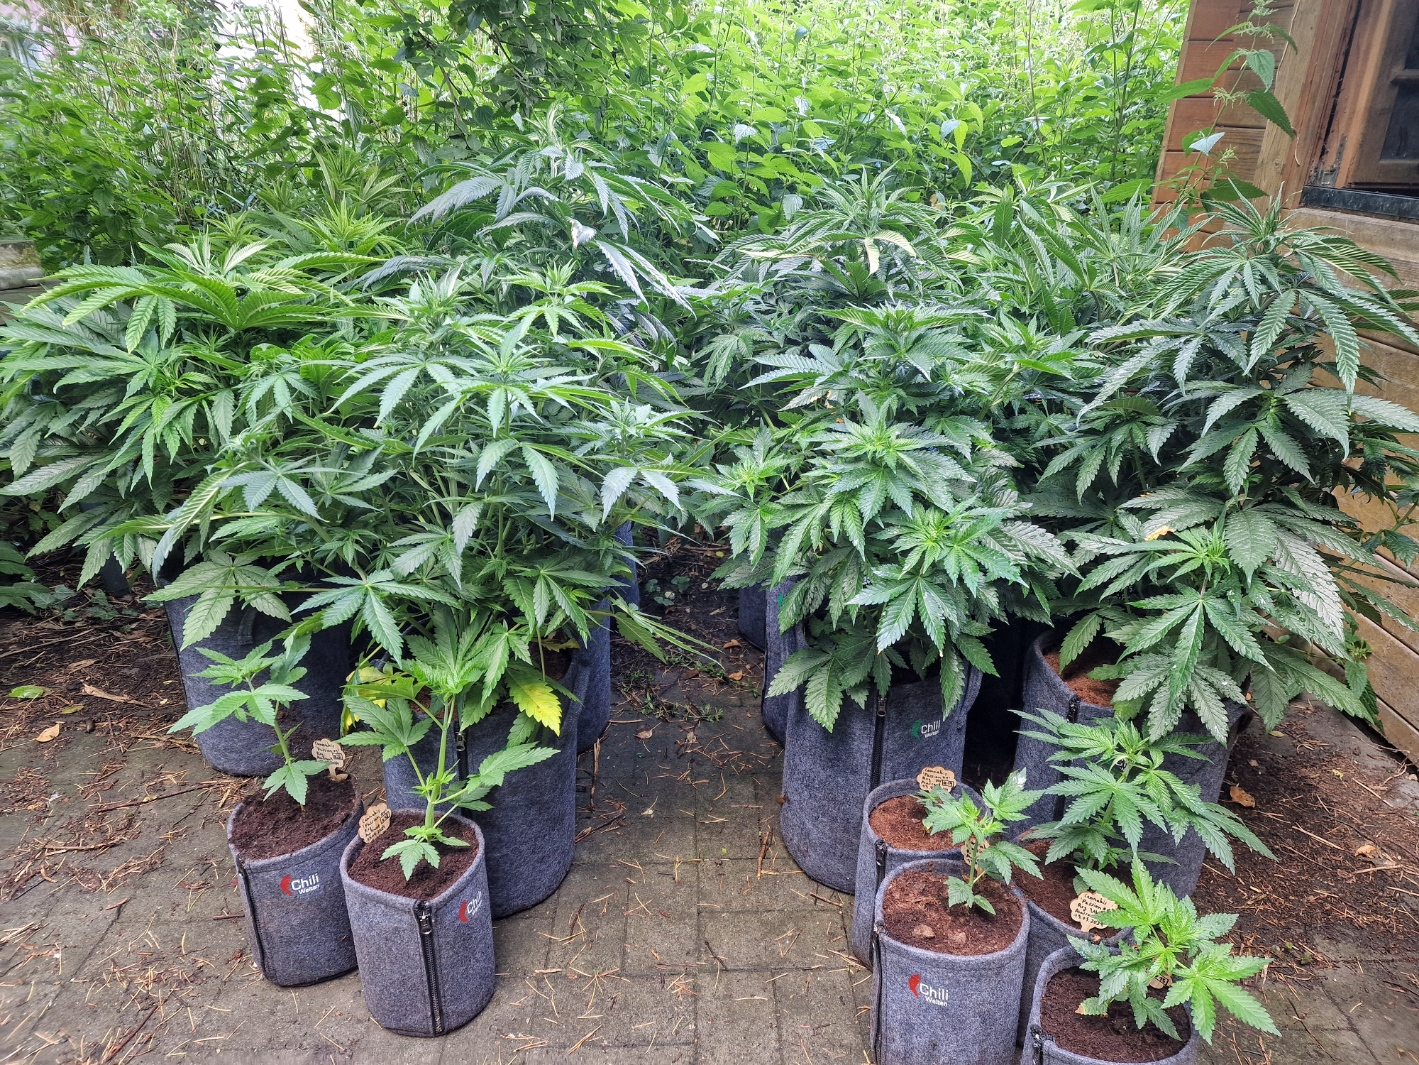
\includegraphics[width=\linewidth]{plant_all_2024-06-17}
            \end{column}
            \begin{column}[T]{.45\textwidth}
                \begin{itemize}
                    \item Has significant economic and medicinal interest
                    \item Cultivated for fiber (hemp), seed oil, and pharmacologically active compounds like cannabinoids and terpenes
                    \item Most notable compounds:
                    \begin{itemize}
                        \item Tetrahydrocannabinol (THC)
                        \item Cannabidiol (CBD)
                    \end{itemize}
               \end{itemize}
            \end{column}
        \end{columns}
    \end{frame}

    \begin{frame}
        \frametitle{The role of light for plants}
        \begin{columns}[t]
            \begin{column}[T]{.55\textwidth}
                \begin{figure}
                    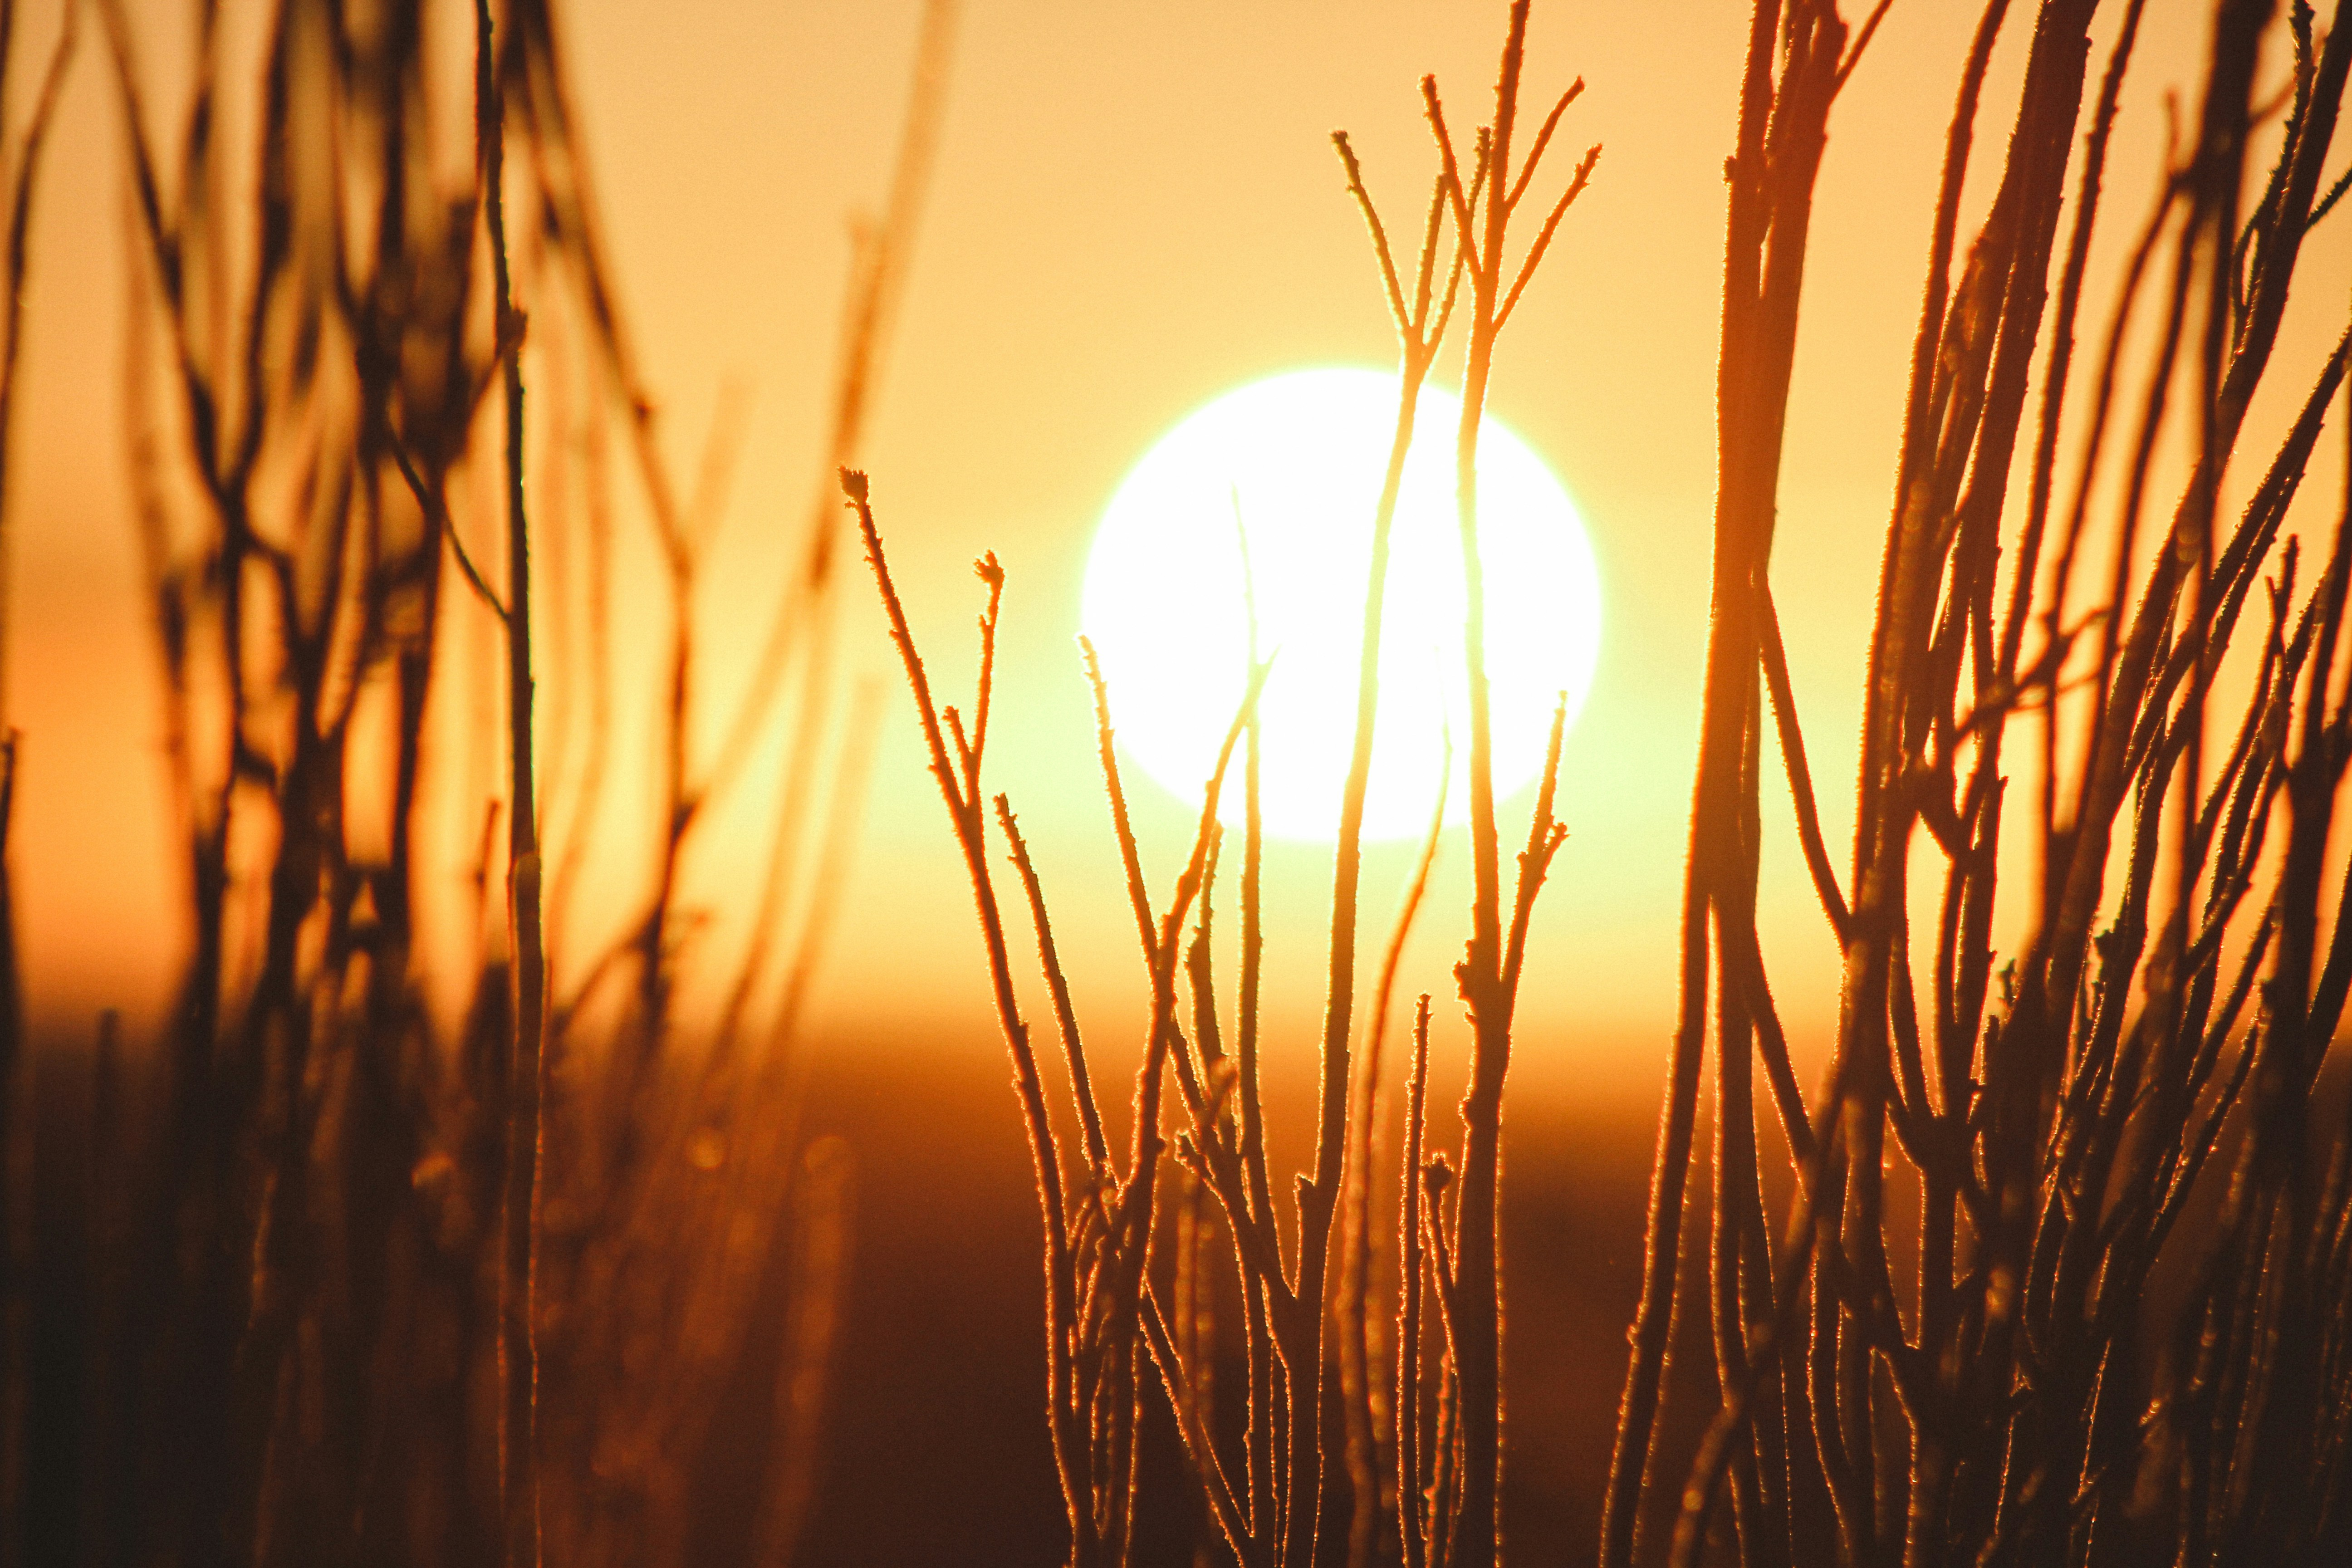
\includegraphics[width=\linewidth]{jeremy-bishop-EdSdhvPX36M-unsplash}
                    \caption{Sunrise. From: \textcite{bishop_foto_2017}}
                \end{figure}
            \end{column}
            \begin{column}[T]{.45\textwidth}
                \begin{itemize}
                    \item Primary energy source for photosynthesis
                    \item Quality and intensity influence growth and development
                    \item Signals the regulation of various physiological processes
                \end{itemize}
                \quad \autocite{eichhorn_bilodeau_update_2019}
            \end{column}
        \end{columns}
    \end{frame}

    \begin{frame}
        \frametitle{And what about UV light?}
        \begin{itemize}
            \item Impact plant growth and secondary metabolite production
            \item UV-A: \qtyrange[mode=text, range-phrase=\textendash, range-units=single]{315}{400}{\nm}
            \item UV-B: \qtyrange[mode=text, range-phrase=\textendash, range-units=single]{280}{315}{\nm}
            \begin{itemize}
                \item Only small proportion in the solar spectrum
                \item Has a higher energy
                \item Causes damage to DNA, proteins, and lipids
                \item Therefore enhances protective secondary metabolites like flavonoids and cannabinoids
                \item In cannabis plants: increases Δ9-tetrahydrocannabinol (THC) production
            \end{itemize}
        \end{itemize}
        \quad \autocite{eichhorn_bilodeau_update_2019, international_organization_for_standardization_space_2007, lydon_uv-b_1987}
    \end{frame}

    \begin{frame}
        \frametitle{Research question and hypothesis}
        \begin{footnotesize}
            \begin{block}{Research question}
                What is the impact of artificial UV light on the germination and seedling development of cannabis seeds?
            \end{block}
            \begin{block}{Hypothesis}
                Exposure to UV light at controlled low intensities would enhance the germination rate and seedling development of cannabis seeds by inducing protective and growth-promoting biochemical responses.
            \end{block}
            \begin{block}{Quantified parameter}
                The treatment group was exposed to additional UV light, the control group not.
            \end{block}
            \begin{block}{Measured parameters}
                \begin{itemize}
                    \item Plant height
                    \item Stem circumference
                    \item Number of internodes
                \end{itemize}
            \end{block}
        \end{footnotesize}
    \end{frame}

    \begin{frame}
        \frametitle{Materials}
        \footnotesize
        \begin{table}
            \begin{tabular}{l|l}
                \hline
                \hline
                \textbf{Item} & \textbf{Description} \\
                \hline
                \hline
                Seeds               & 2 seeds of DUTCH PASSION Skywalker Haze (feminized) \\
                                    & 10 seeds of DUTCH PASSION Frisian Dew seeds (feminized) \\
                \bigstrut
                Planting containers & \qty[mode=text]{3}{\L} fabric planting containers from Chiliwelten with zipper \\
                                    & \qty[mode=text]{15}{\L} fabric planting containers from Chiliwelten with zipper \\
                \bigstrut
                Potting soil        & Lightly fertilized organic coconut potting soil \\
                                    & with added mycorrhizae (for seeds) \\
                                    & Fertilized organic coconut potting soil (for potting up) \\
                \bigstrut
                LED Grow lights     & PHLIZON FD6000 PLUS 640W Full-spectrum Daisy Chain \\
                                    & Dimmable LED Grow Light \\
                \bigstrut
                UV grow lights      & LuxElite PlantUV (fluorescent tube, \qty[mode=text]{24}{\W}, color temp. \qty[mode=text]{7000}{\K}) \\
                                    & \quad UV-A: \qty[mode=text]{30}{\percent} \\
                                    & \quad UV-B: \qty[mode=text]{12}{\percent} \\
                \bigstrut
                Light spectrometer  & THORLABS CCS200/M \\
                                    & \quad Wavelengths: \qtyrange[mode=text, range-phrase=\textendash, range-units=single]{200}{1000}{\nm} \\
                \hline
                \hline
            \end{tabular}
        \end{table}
    \end{frame}

    \begin{frame}
        \frametitle{The cannabis seeds 'Skywalker Haze'}
        \begin{figure}
            \begin{subfigure}[t]{.48\textwidth}
                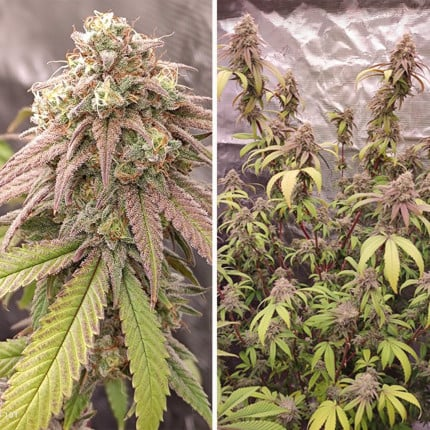
\includegraphics[width=\linewidth]{DUTCH-PASSION_Skywalker-Haze_1}
            \end{subfigure}
            \hfill
            \begin{subfigure}[t]{.48\textwidth}
                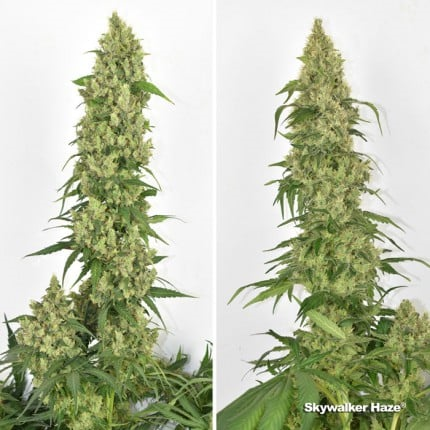
\includegraphics[width=\linewidth]{DUTCH-PASSION_Skywalker-Haze_2}
            \end{subfigure}
            \caption{DUTCH PASSION Skywalker Haze cultivar. From: \textcite{noauthor_dutch-passion_skywalker-haze_nodate}}
        \end{figure}
    \end{frame}

    \begin{frame}
        \frametitle{The cannabis seeds 'Frisian Dew'}
        \begin{figure}
            \begin{subfigure}[t]{.48\textwidth}
                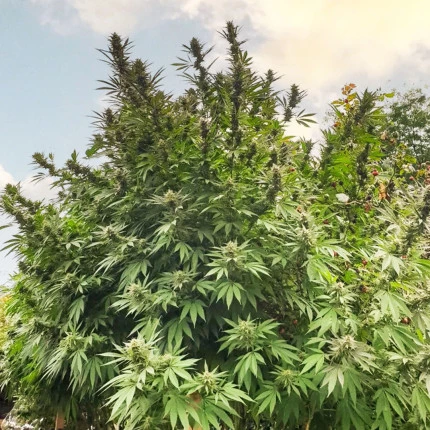
\includegraphics[width=\linewidth]{DUTCH-PASSION_Frisian-Dew_1}
            \end{subfigure}
            \hfill
            \begin{subfigure}[t]{.48\textwidth}
                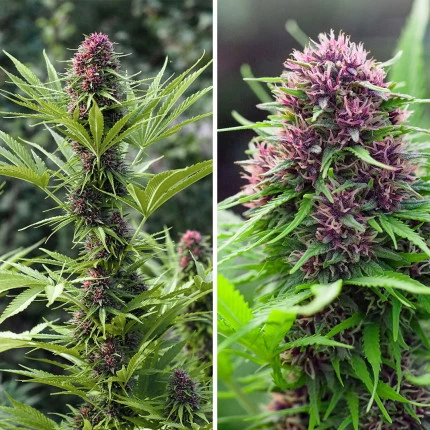
\includegraphics[width=\linewidth]{DUTCH-PASSION_Frisian-Dew_2}
            \end{subfigure}
            \caption{DUTCH PASSION Frisian Dew cultivar. From: \textcite{noauthor_dutch-passion_frisian-dew_nodate}}
        \end{figure}
    \end{frame}

    \begin{frame}
        \frametitle{The planting containers}
        \begin{figure}
            \begin{subfigure}[t]{.48\textwidth}
                \includegraphics[width=\linewidth]{Chiliwelten_3L-Stofftopf-Reißverschluss}
                \subcaption{\qty[mode=text]{3}{\L} planting container. From: \textcite{noauthor_chiliwelten_3l_nodate}}
            \end{subfigure}
            \hfill
            \begin{subfigure}[t]{.48\textwidth}
                \includegraphics[width=\linewidth]{Chiliwelten_15L-Stofftopf-Reißverschluss}
                \subcaption{\qty[mode=text]{15}{\L} planting container. From: \textcite{noauthor_chiliwelten_15l_nodate}}
            \end{subfigure}
        \end{figure}
    \end{frame}

    \begin{frame}
        \frametitle{The LED grow lights}
        \begin{figure}
            \begin{subfigure}[t]{.48\textwidth}
                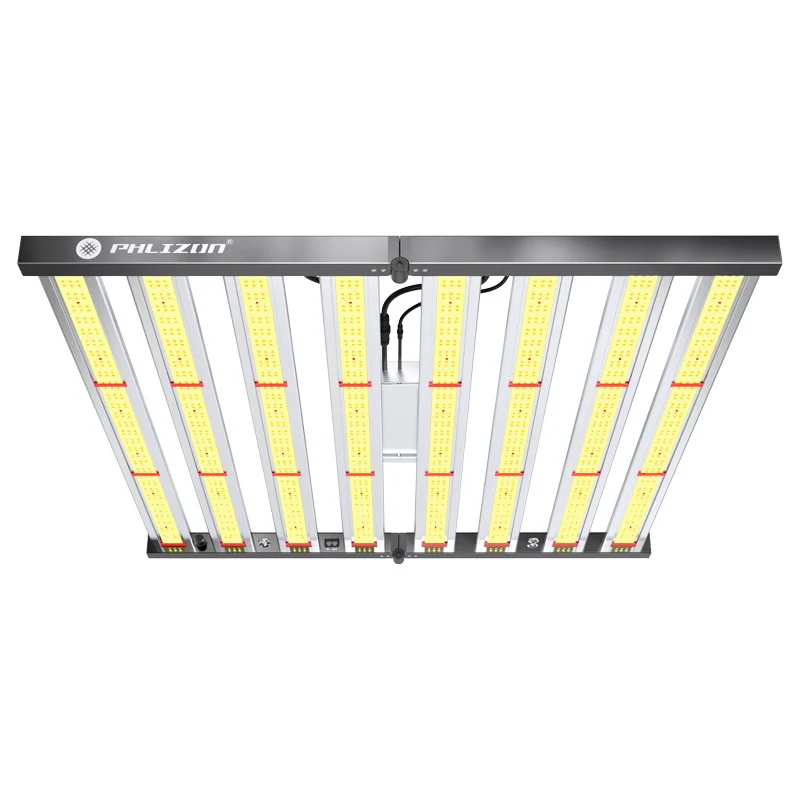
\includegraphics[width=\linewidth]{PHLIZON_PH-FD8-E}
            \end{subfigure}
            \hfill
            \begin{subfigure}[t]{.42\textwidth}
                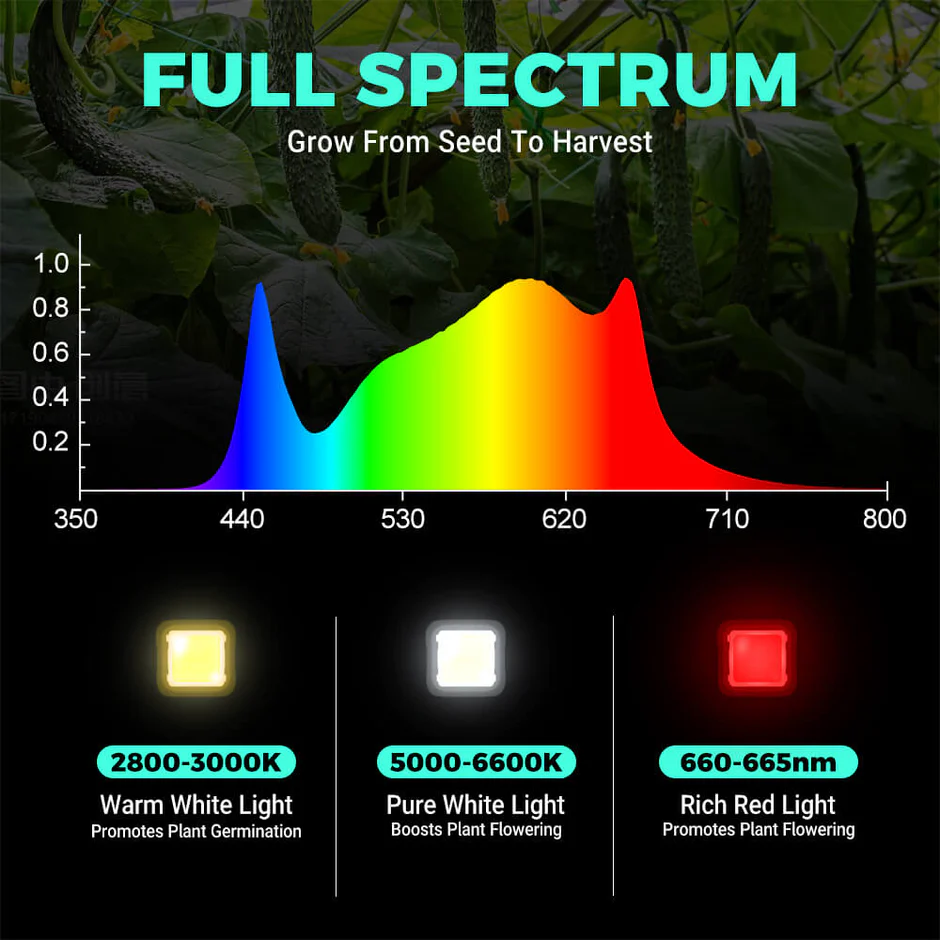
\includegraphics[width=\linewidth]{PHLIZON_PH-FD8-E_light-spectrum}
            \end{subfigure}
            \caption{LED grow light. From: \textcite{noauthor_phlizon_fd6000-640w-upgraded_nodate}}
        \end{figure}
    \end{frame}

    \begin{frame}
        \frametitle{The UV grow lights}
        \begin{figure}
            \begin{subfigure}[t]{.48\textwidth}
                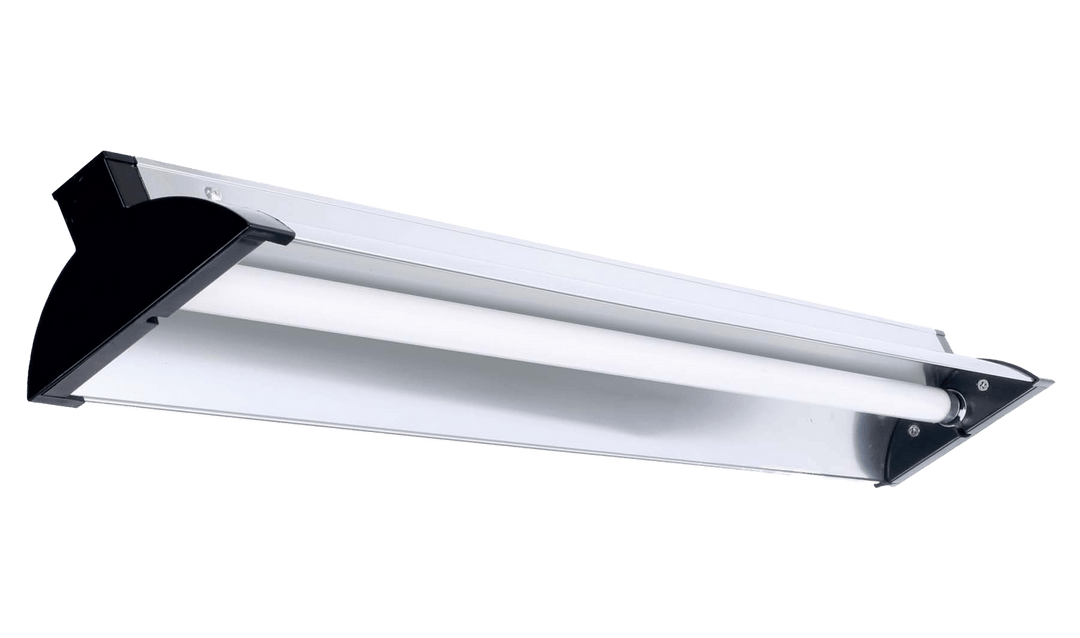
\includegraphics[width=\linewidth]{LuxElite_PlantUV}
            \end{subfigure}
            \hfill
            \begin{subfigure}[t]{.48\textwidth}
                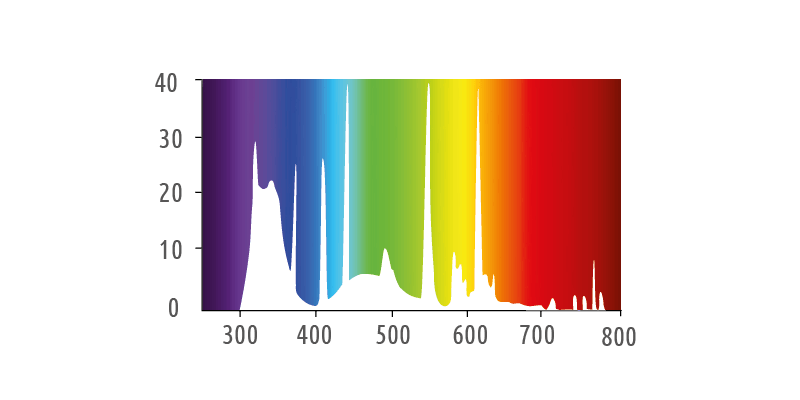
\includegraphics[width=\linewidth]{LuxElite_PlantUV_light-spectrum}
            \end{subfigure}
            \caption{UV grow light. From: \textcite{noauthor_luxelite_plantuv_nodate}}
        \end{figure}
    \end{frame}

    \begin{frame}
        \frametitle{The light spectra}
        \begin{figure}
            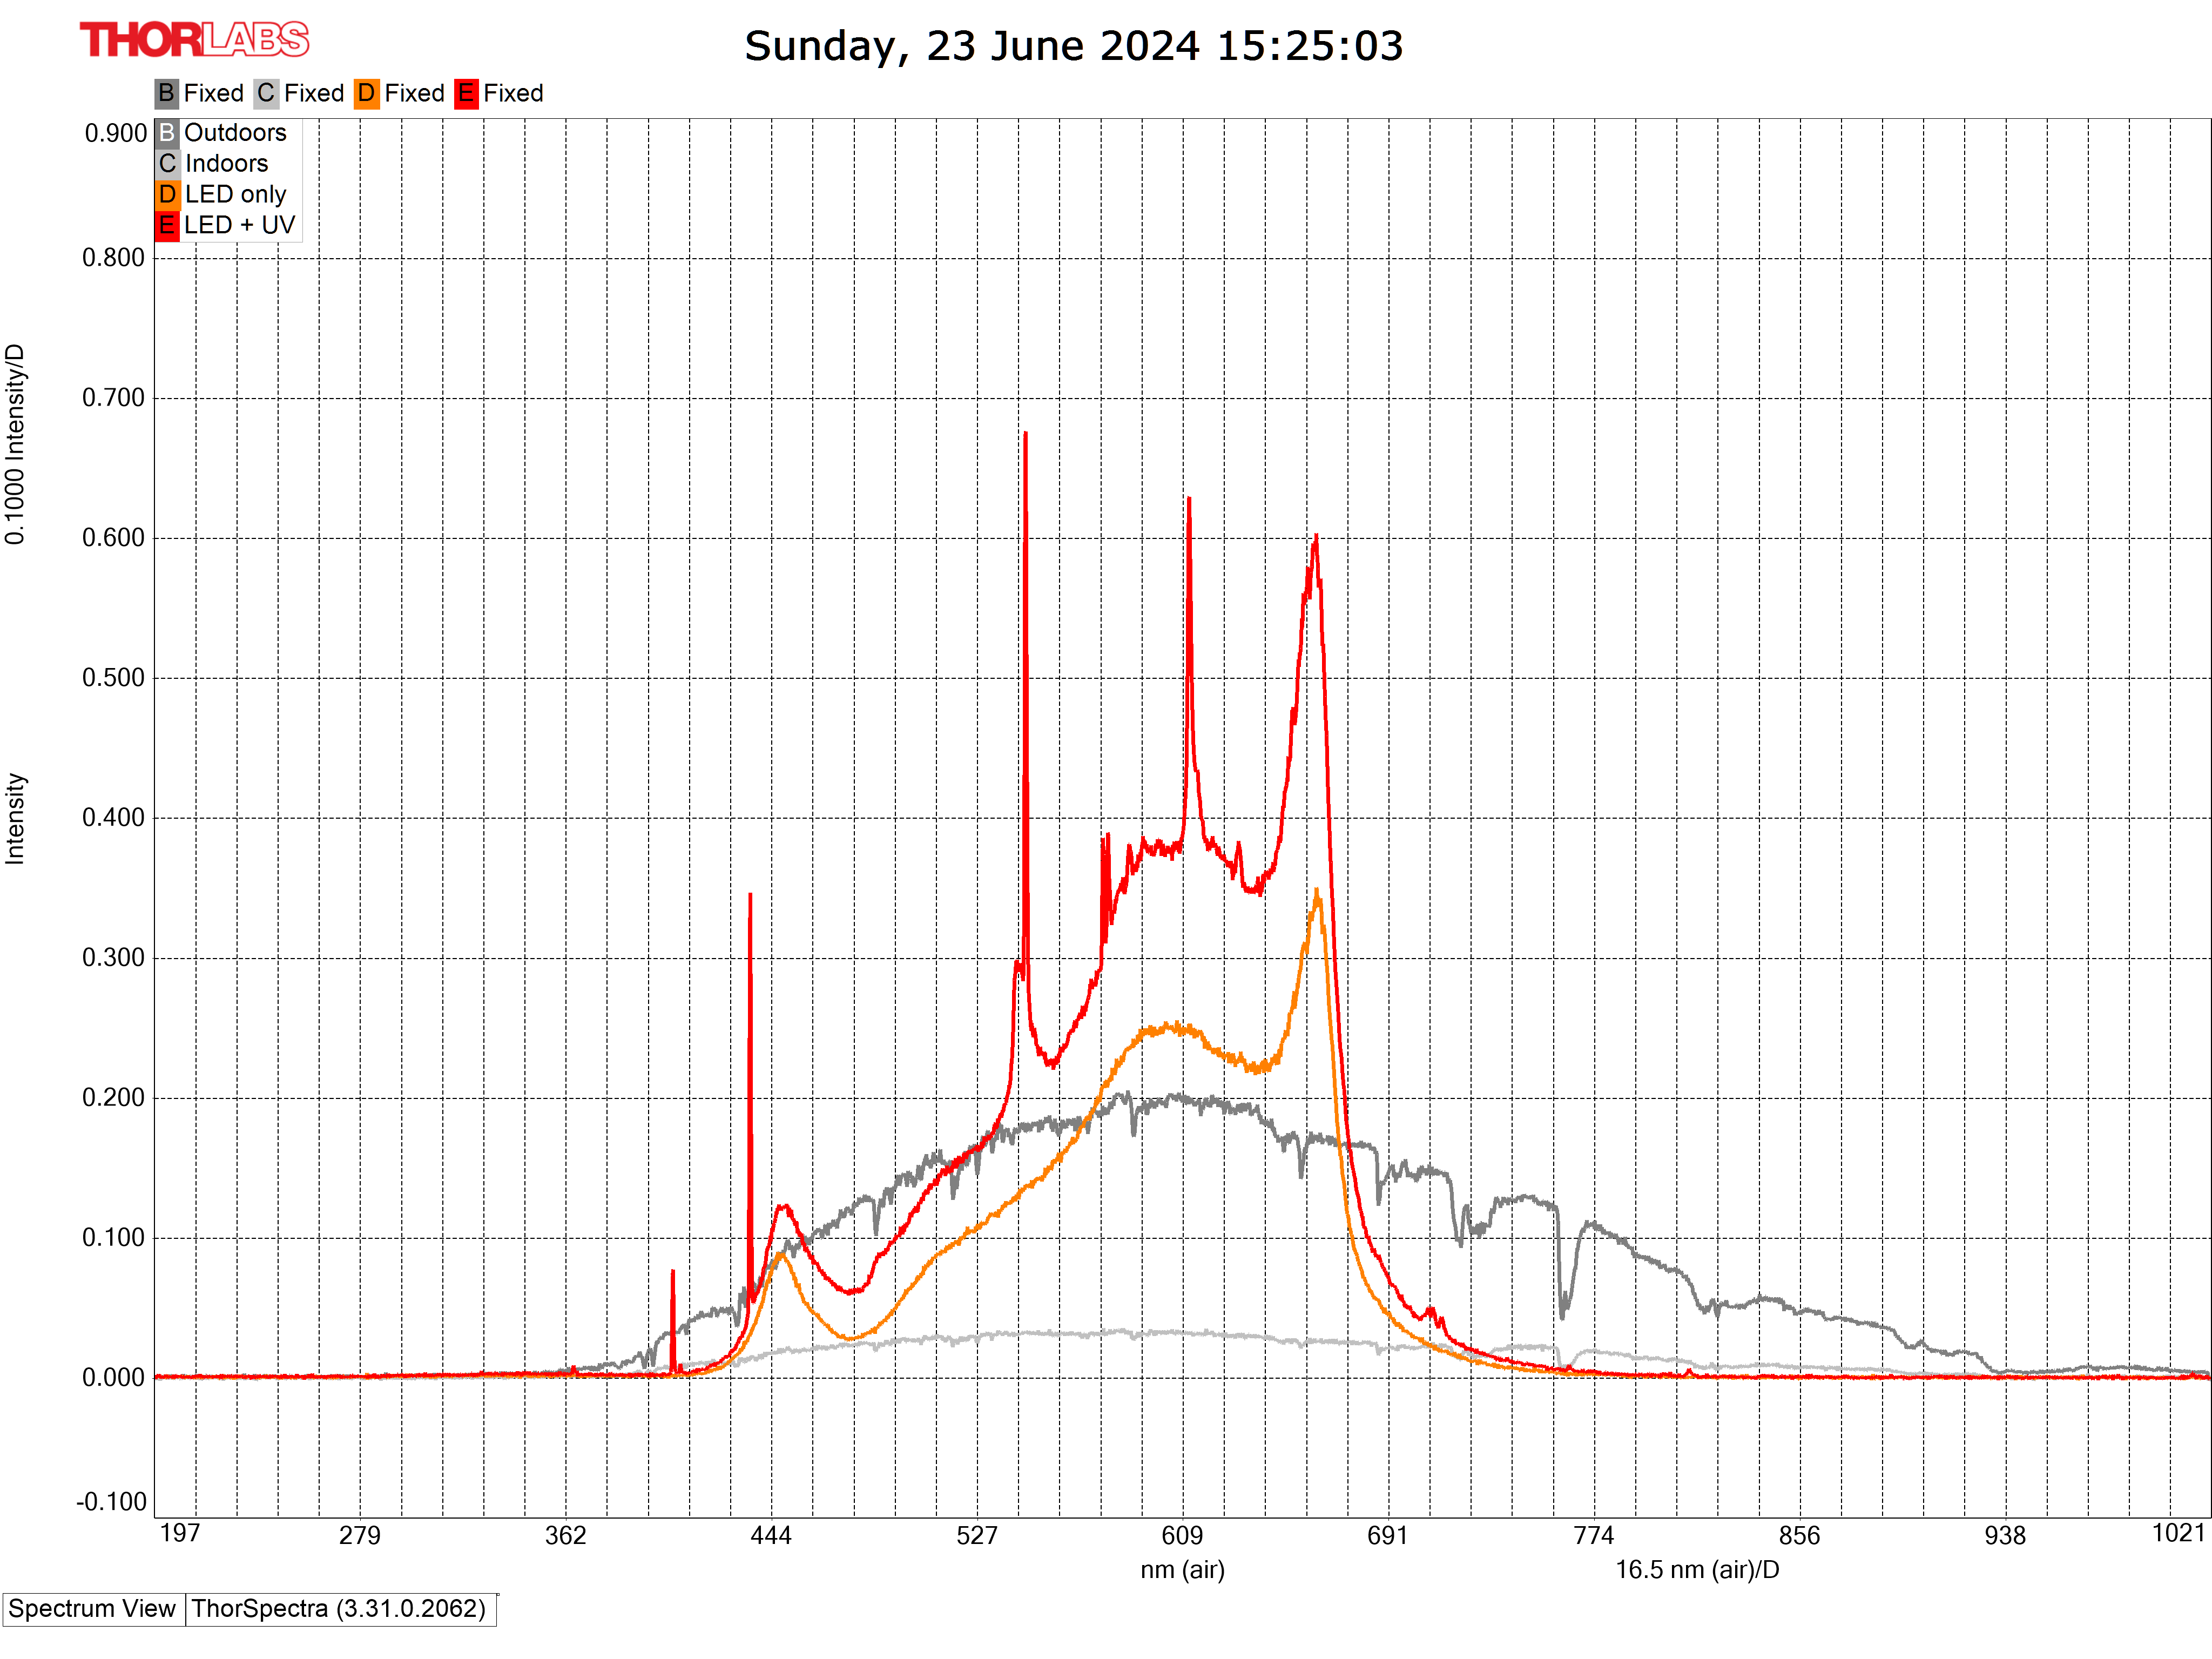
\includegraphics[width=0.6\linewidth]{light-spectra_outdoors_indoors_led_led+uv}
            \caption{Light spectra of the experimental setups with LED grow lights only (control) and with additional UV fluorescent tubes, as well as the spectra measured outdoors and indoors.}
        \end{figure}
    \end{frame}

    \begin{frame}
        \frametitle{Experimental procedure}
        \begin{figure}
            \begin{tikzpicture}[node distance=1.6cm]
                % Define styles
                \tikzstyle{box_all_groups} = [font=\scriptsize , rectangle, draw, fill=gray!40, text width=12em, text centered, rounded corners, minimum height=2.85em]
                \tikzstyle{box_ctrl_group} = [font=\scriptsize, rectangle, draw, fill=green!40, text width=12em, text centered, rounded corners, minimum height=2.85em]
                \tikzstyle{box_exp_group} = [font=\scriptsize, rectangle, draw, fill=pink!40, text width=12em, text centered, rounded corners, minimum height=2.85em]
                \tikzstyle{line} = [draw, -latex]

                % Nodes
                \node [box_all_groups] (start) {Start: May 2};

                \node [box_ctrl_group, below of=start] (ctrl_group_start) {Group 1 (Control): LED lights only};
                \node [box_exp_group, right of=ctrl_group_start, node distance=6cm] (exp_group_start) {Group 2: LED + UV lights};

                \node [box_ctrl_group, below of=ctrl_group_start] (ctrl_group_seed) {Plant  1 seed of Skywalker Haze (feminized) and 5 seeds of Frisian Dew (feminized)};
                \node [box_exp_group, below of=exp_group_start] (exp_group_seed) {Plant  1 seed of Skywalker Haze (feminized) and 5 seeds of Frisian Dew (feminized)};

                \node [box_ctrl_group, below of=ctrl_group_seed] (ctrl_group_transplant) {Transplant to \qty[mode=text]{15}{\L} pots on May 13};
                \node [box_exp_group, below of=exp_group_seed] (exp_group_transplant) {Transplant to \qty[mode=text]{15}{\L} pots on May 13};

                \node [box_all_groups, ultra thick, below of=ctrl_group_transplant] (assess) {Assess growth parameters on June 17};

                % Lines
                \path [line] (start) -- (ctrl_group_start);
                \path [line] (start) -- (exp_group_start);

                \path [line] (ctrl_group_start) -- (ctrl_group_seed);
                \path [line] (exp_group_start) -- (exp_group_seed);

                \path [line] (ctrl_group_seed) -- (ctrl_group_transplant);
                \path [line] (exp_group_seed) -- (exp_group_transplant);

                \path [line] (ctrl_group_transplant) -- (assess);
                \path [line] (exp_group_transplant) -- (assess);
            \end{tikzpicture}
        \end{figure}
    \end{frame}

    \begin{frame}
        \frametitle{Growing conditions}
        \begin{itemize}
            \item Temperature \~{} \qty[mode=text]{21}{\degreeCelsius}
            \item Grow lights were adjusted to maintain a distance of \~{} \qty[mode=text]{20}{\cm} from the tip of the tallest plant
            \item LED grow lights were set to \qty[mode=text]{100}{\percent} dimmable intensity
            \item All lights were on daily from 5:35 a.m. to 9:35 p.m. (\qty[mode=text]{16}{hr} daily)
            \item On June 17: sunrise at 5:18 a.m. and sunset at 9:52 p.m.
        \end{itemize}
    \end{frame}

    \begin{frame}
        \frametitle{The plants on May 13}
        \begin{figure}[H]
            \begin{minipage}[t]{0.45\textwidth}
                \begin{subfigure}[t]{.32\textwidth}
                    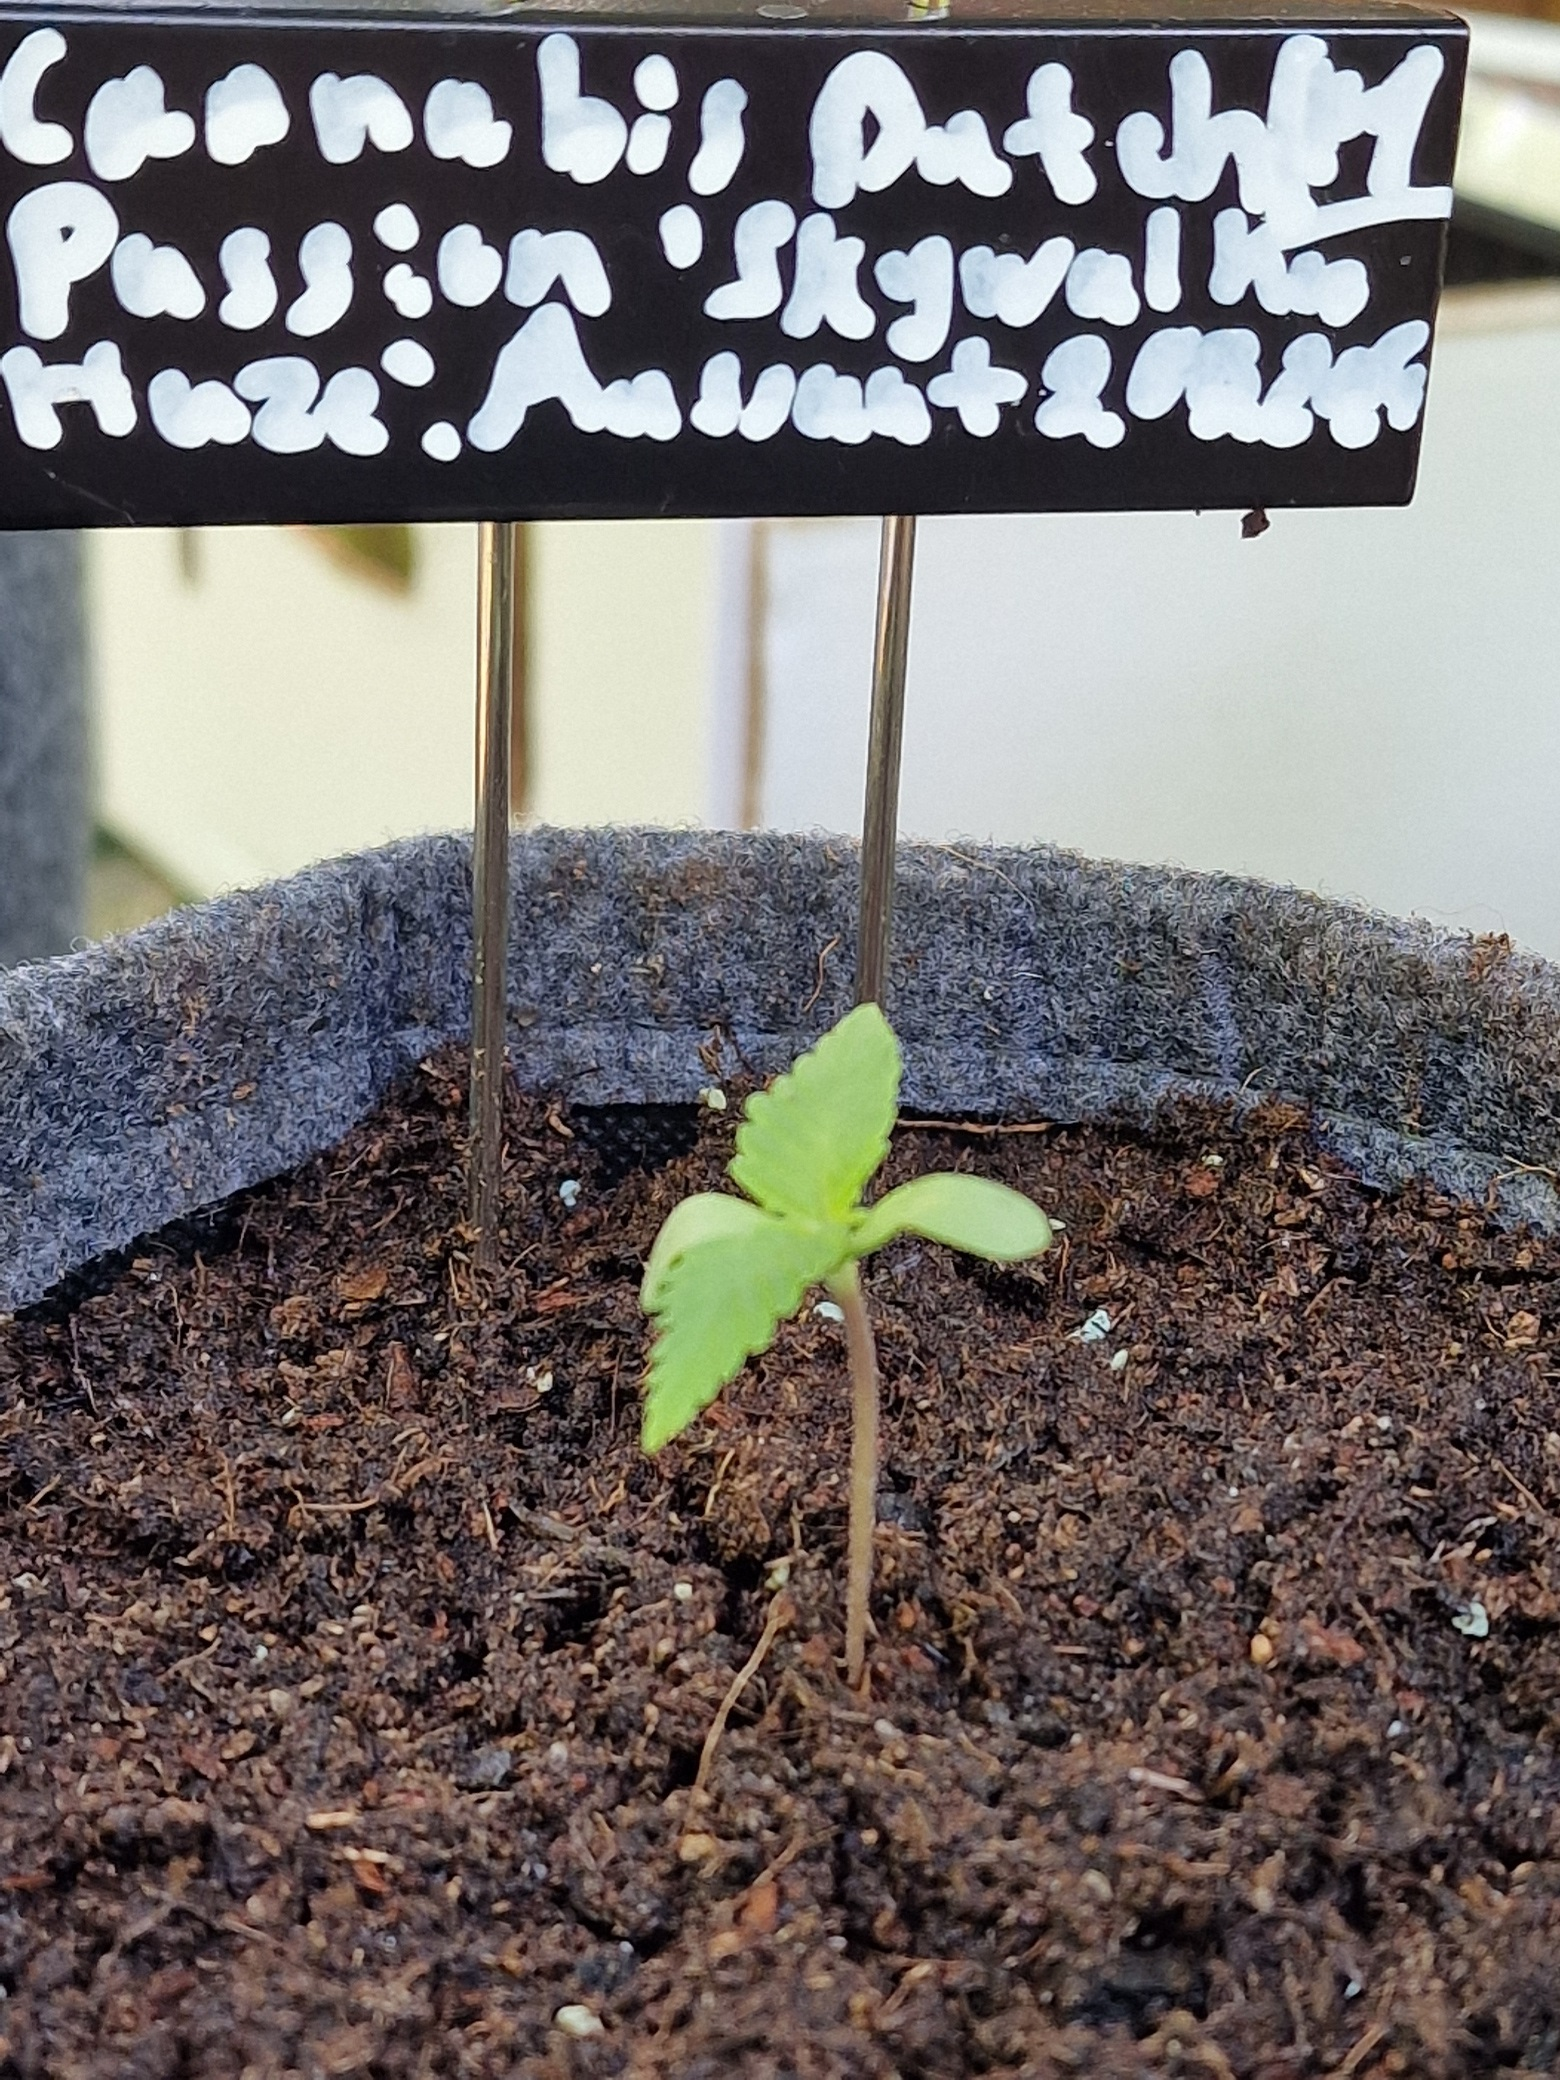
\includegraphics[width=\linewidth]{plant_01_2024-05-13}
                    \subcaption{Plant \#1}
                \end{subfigure}
                \begin{subfigure}[t]{.32\textwidth}
                    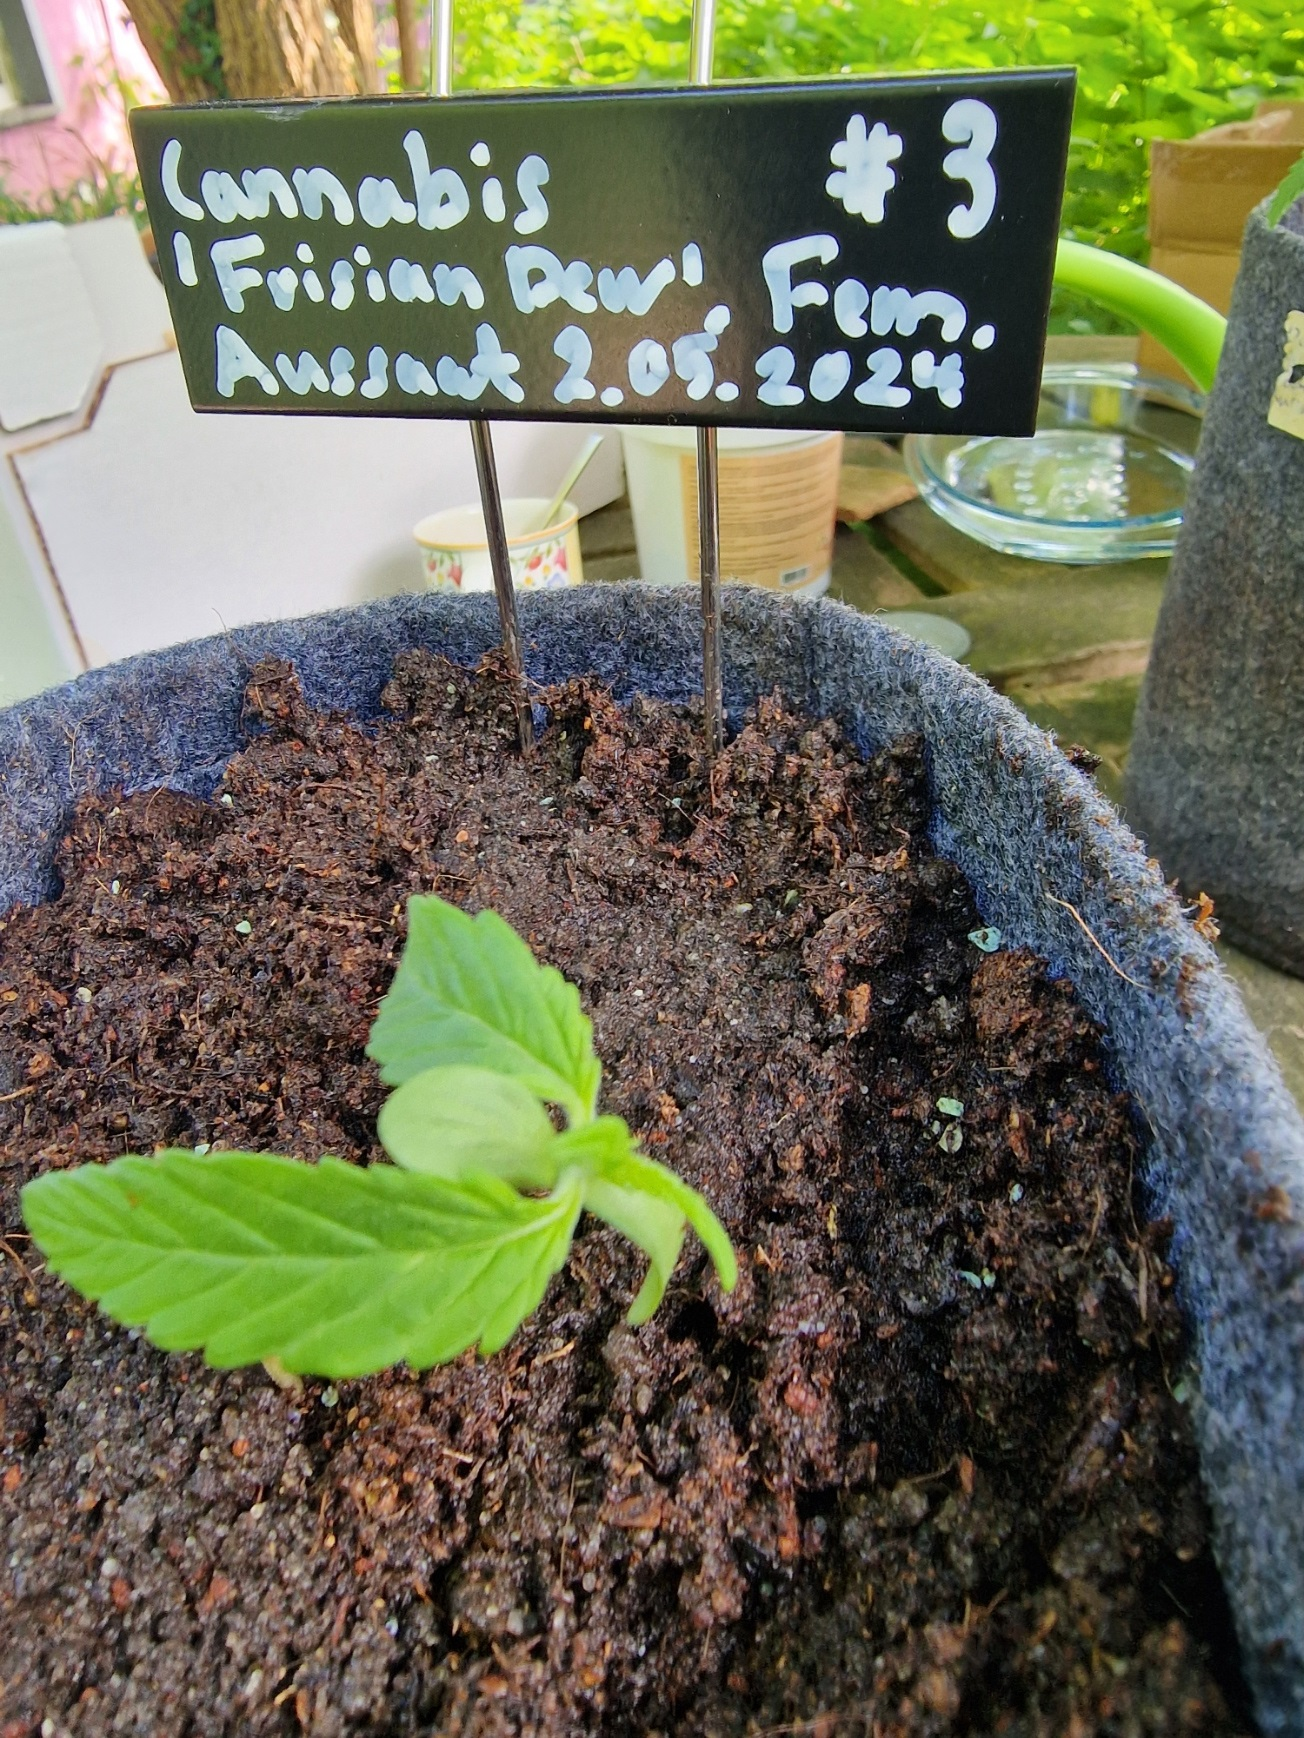
\includegraphics[width=\linewidth]{plant_03_2024-05-13}
                    \subcaption{Plant \#3}
                \end{subfigure}
                \begin{subfigure}[t]{.32\textwidth}
                    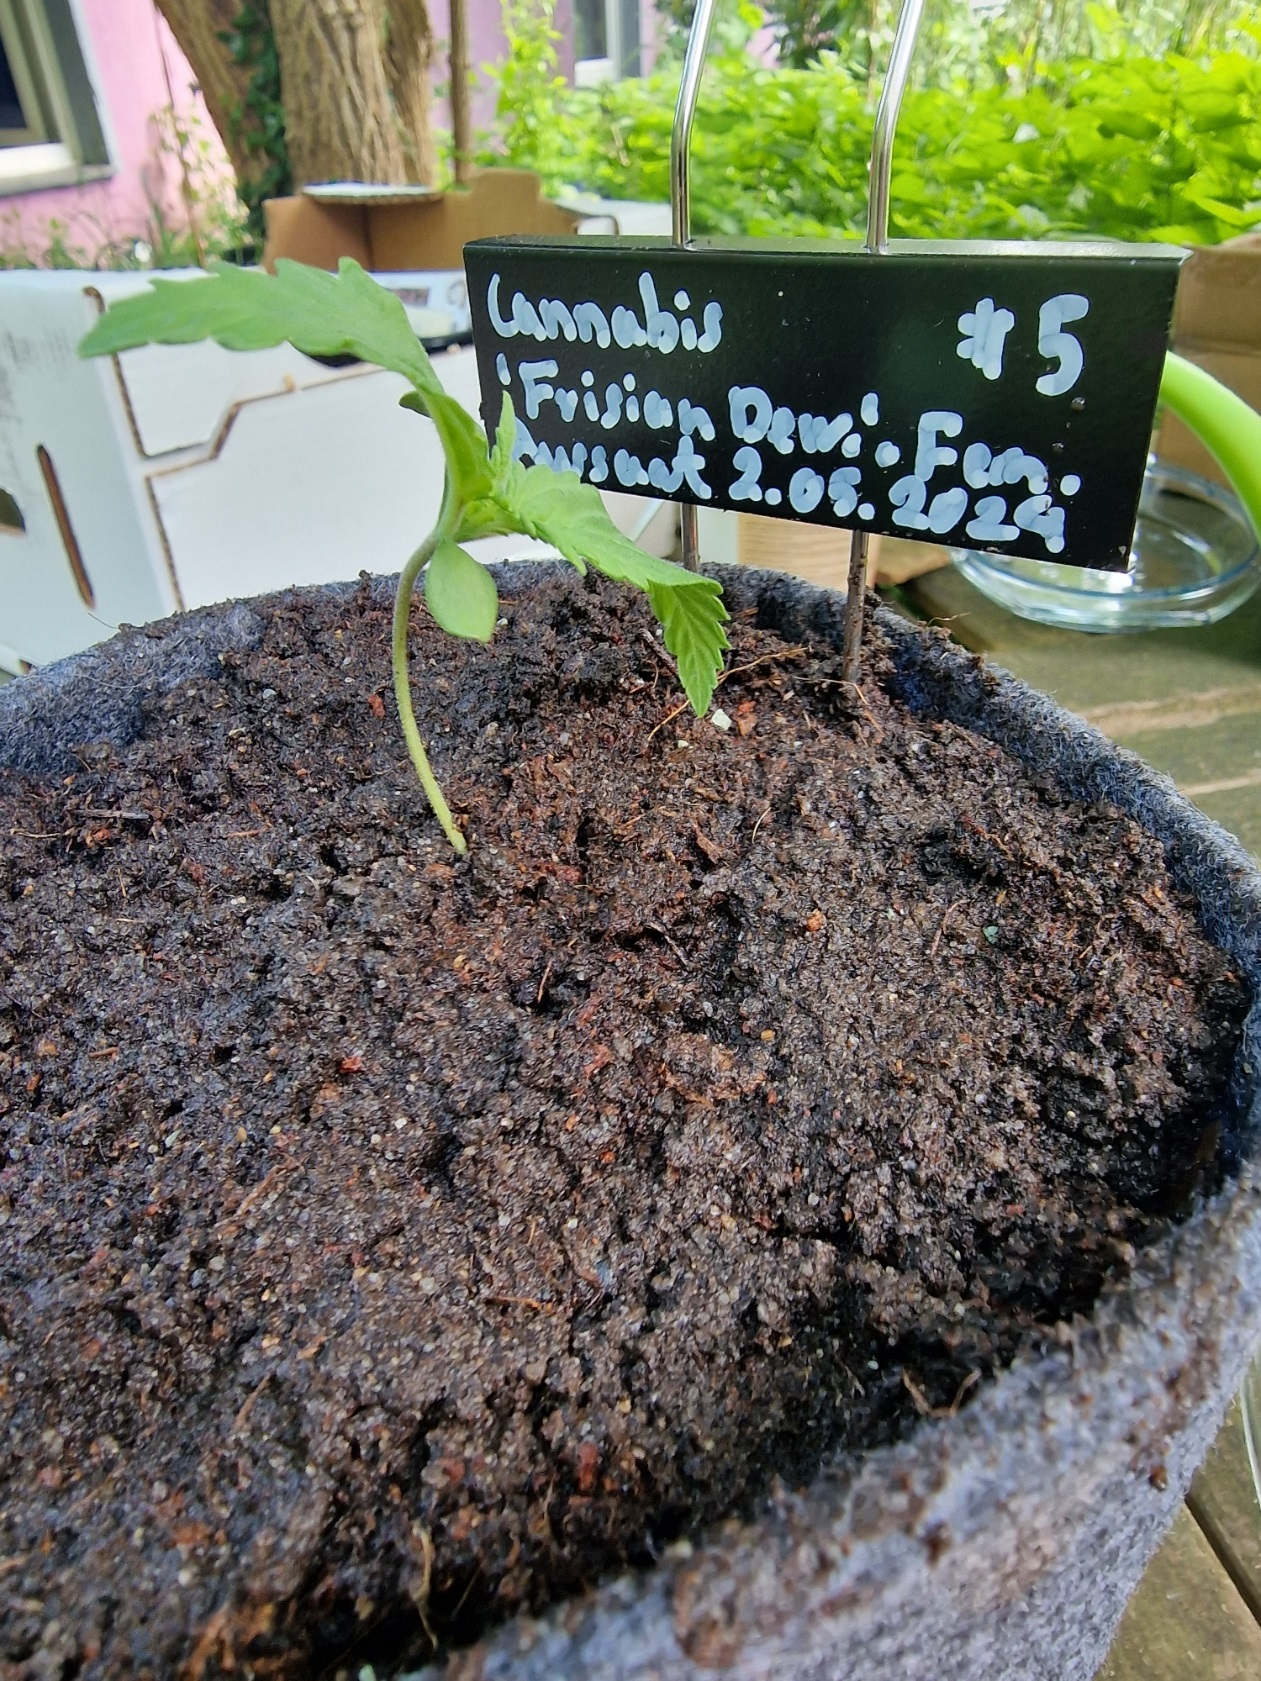
\includegraphics[width=\linewidth]{plant_05_2024-05-13}
                    \subcaption{Plant \#5}
                \end{subfigure}
                \begin{subfigure}[t]{.32\textwidth}
                    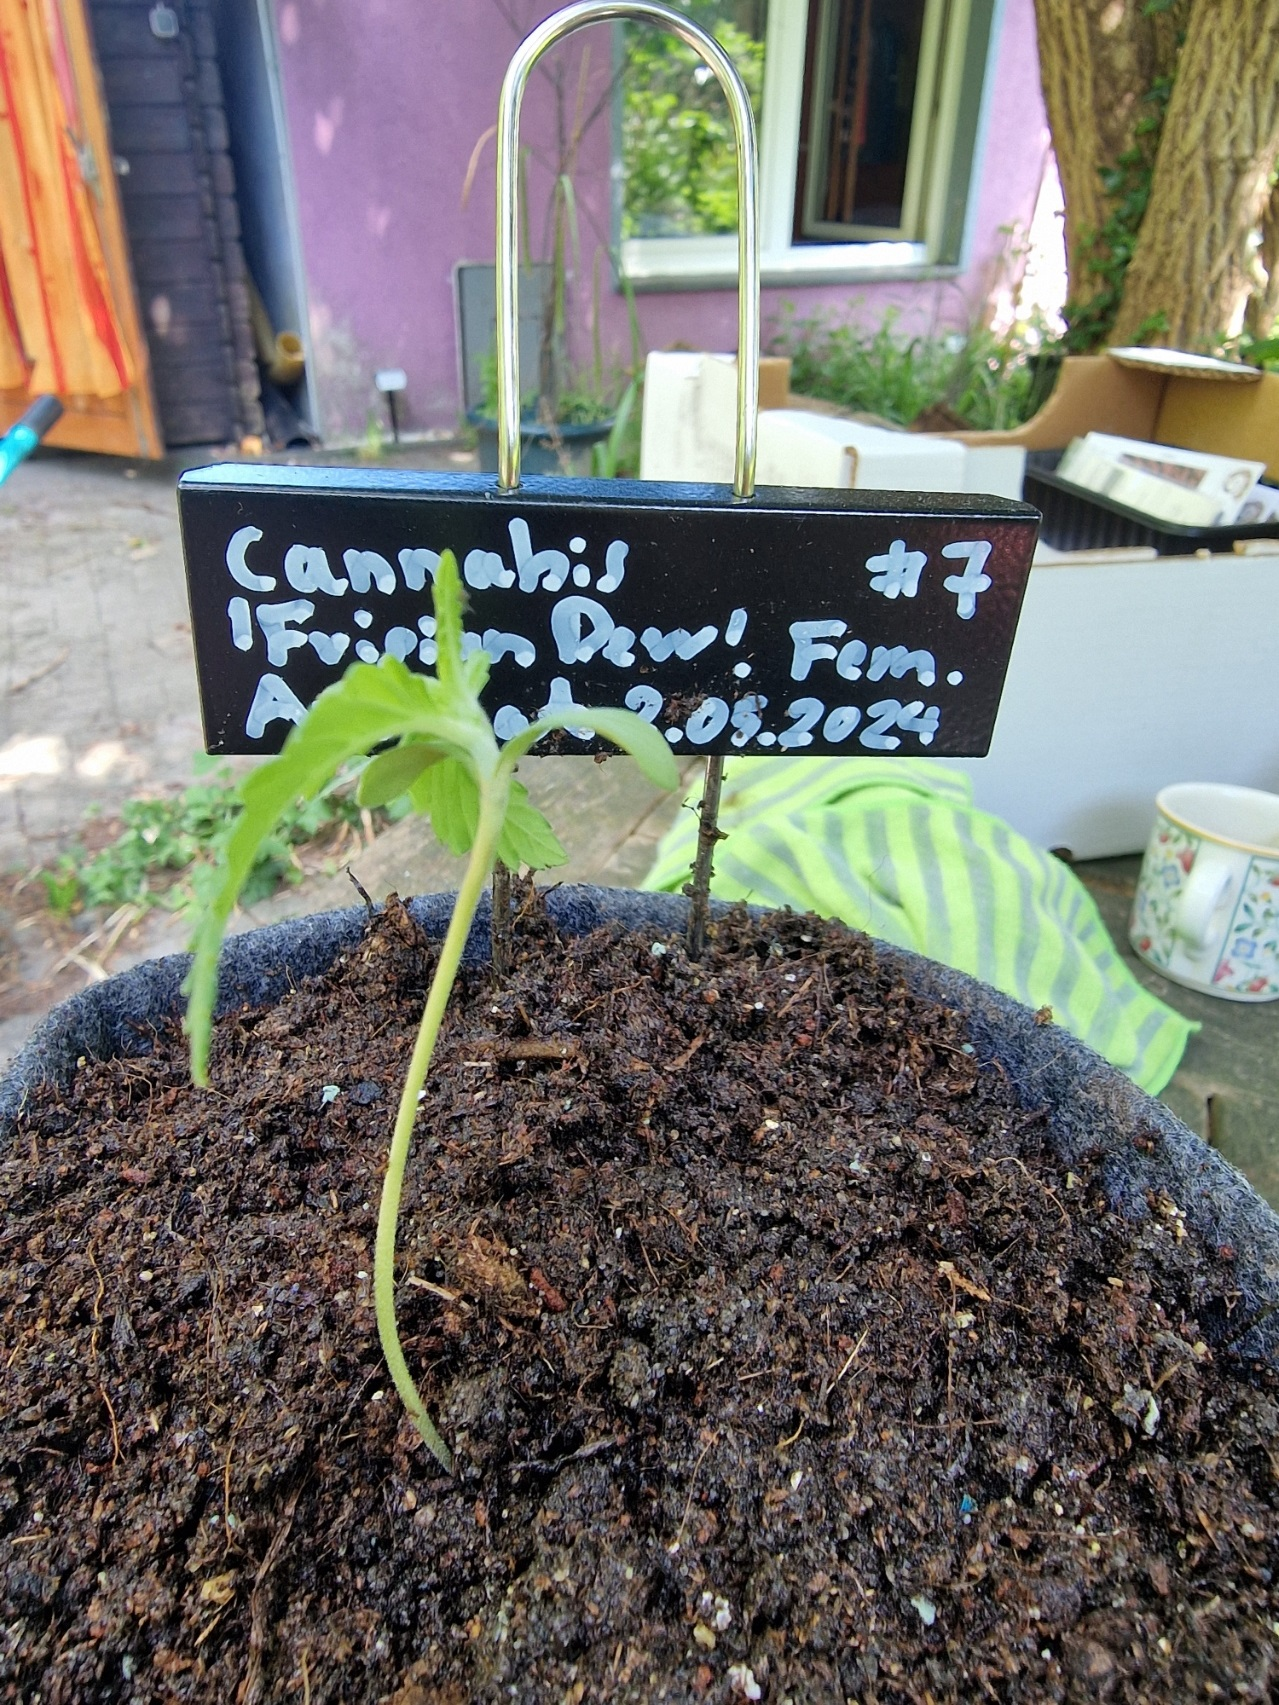
\includegraphics[width=\linewidth]{plant_07_2024-05-13}
                    \subcaption{Plant \#7}
                \end{subfigure}
                \begin{subfigure}[t]{.32\textwidth}
                    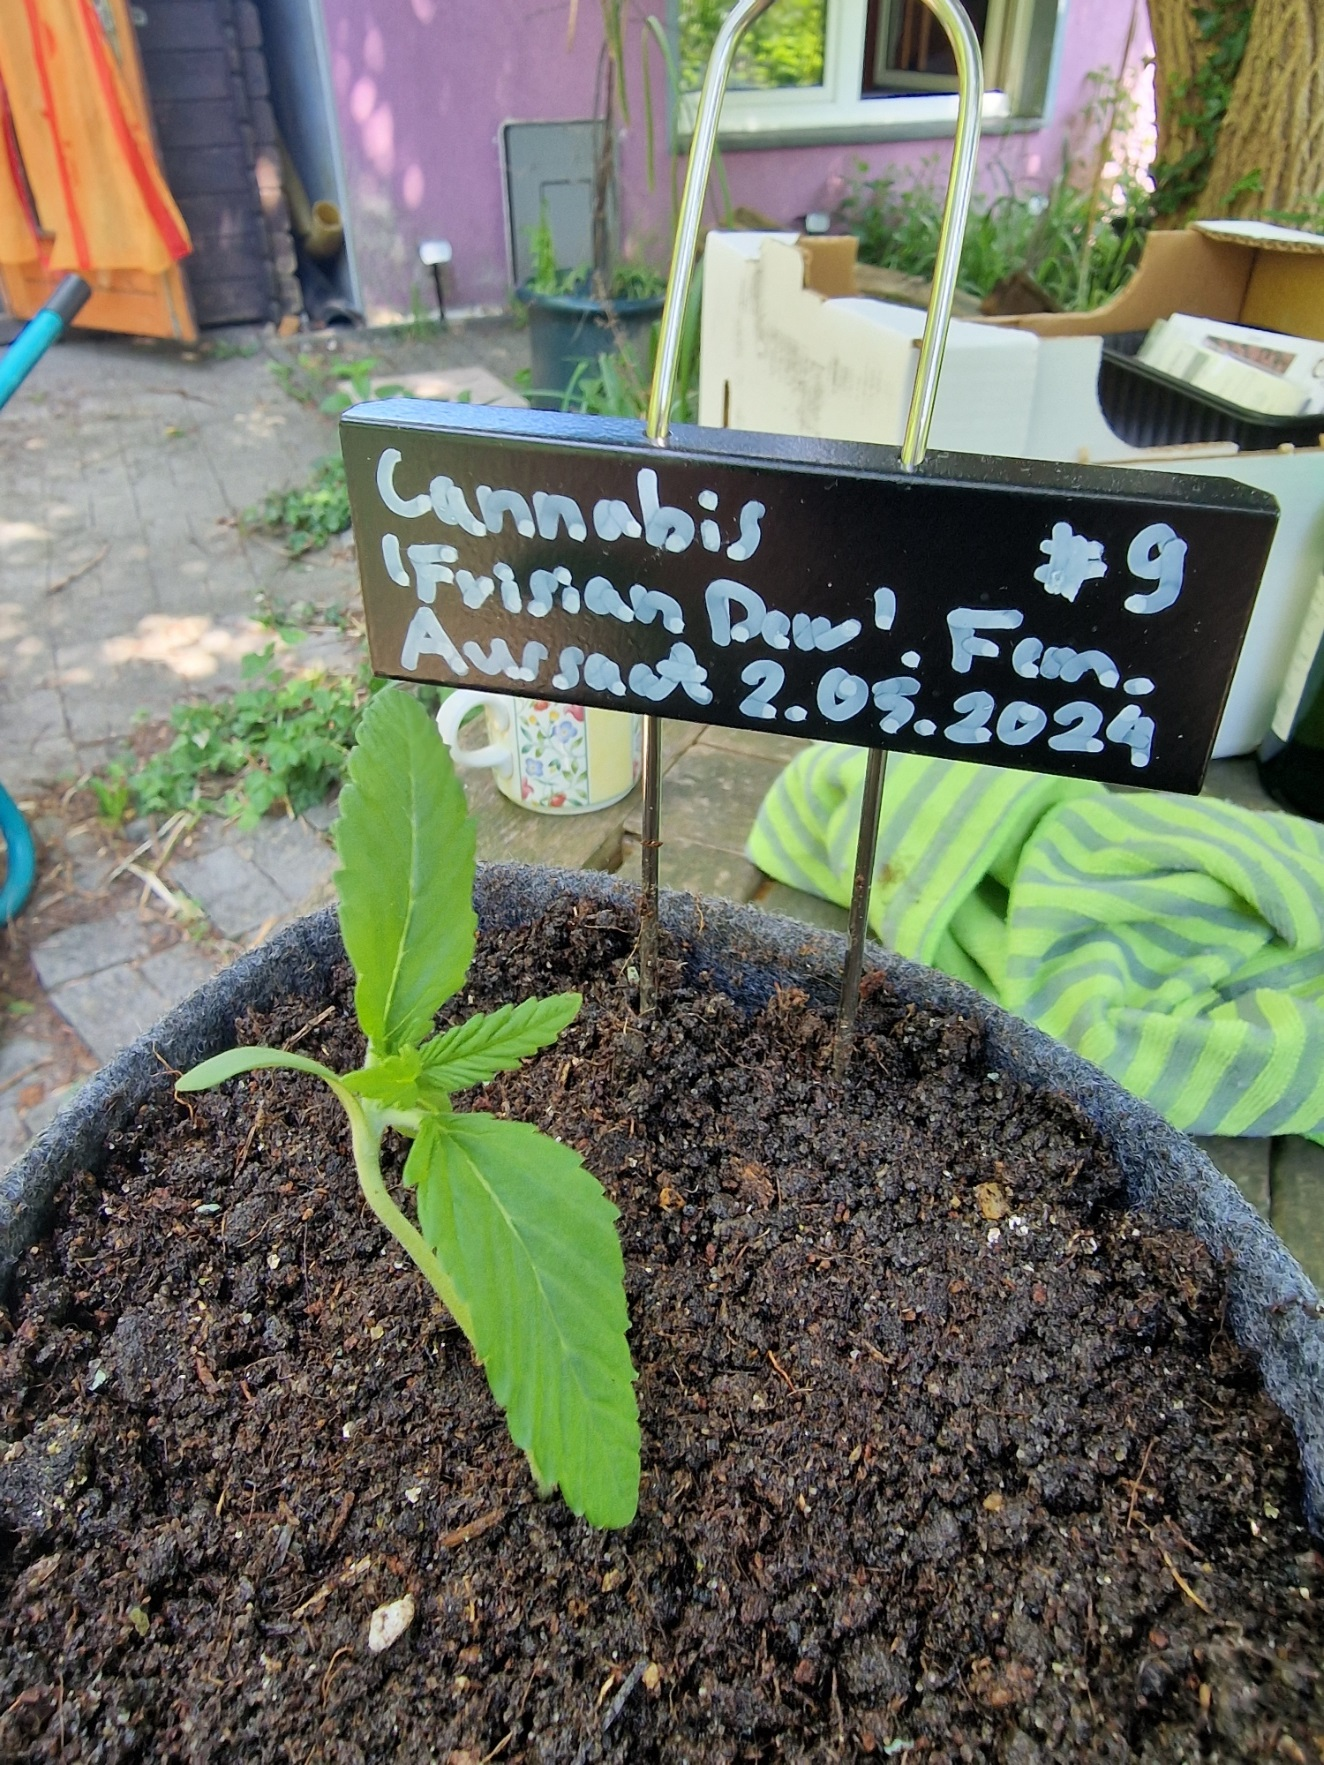
\includegraphics[width=\linewidth]{plant_09_2024-05-13}
                    \subcaption{Plant \#9}
                \end{subfigure}
                \caption{UV group}
            \end{minipage}
            \hfill
            \begin{minipage}[t]{0.45\textwidth}
                \begin{subfigure}[t]{.32\textwidth}
                    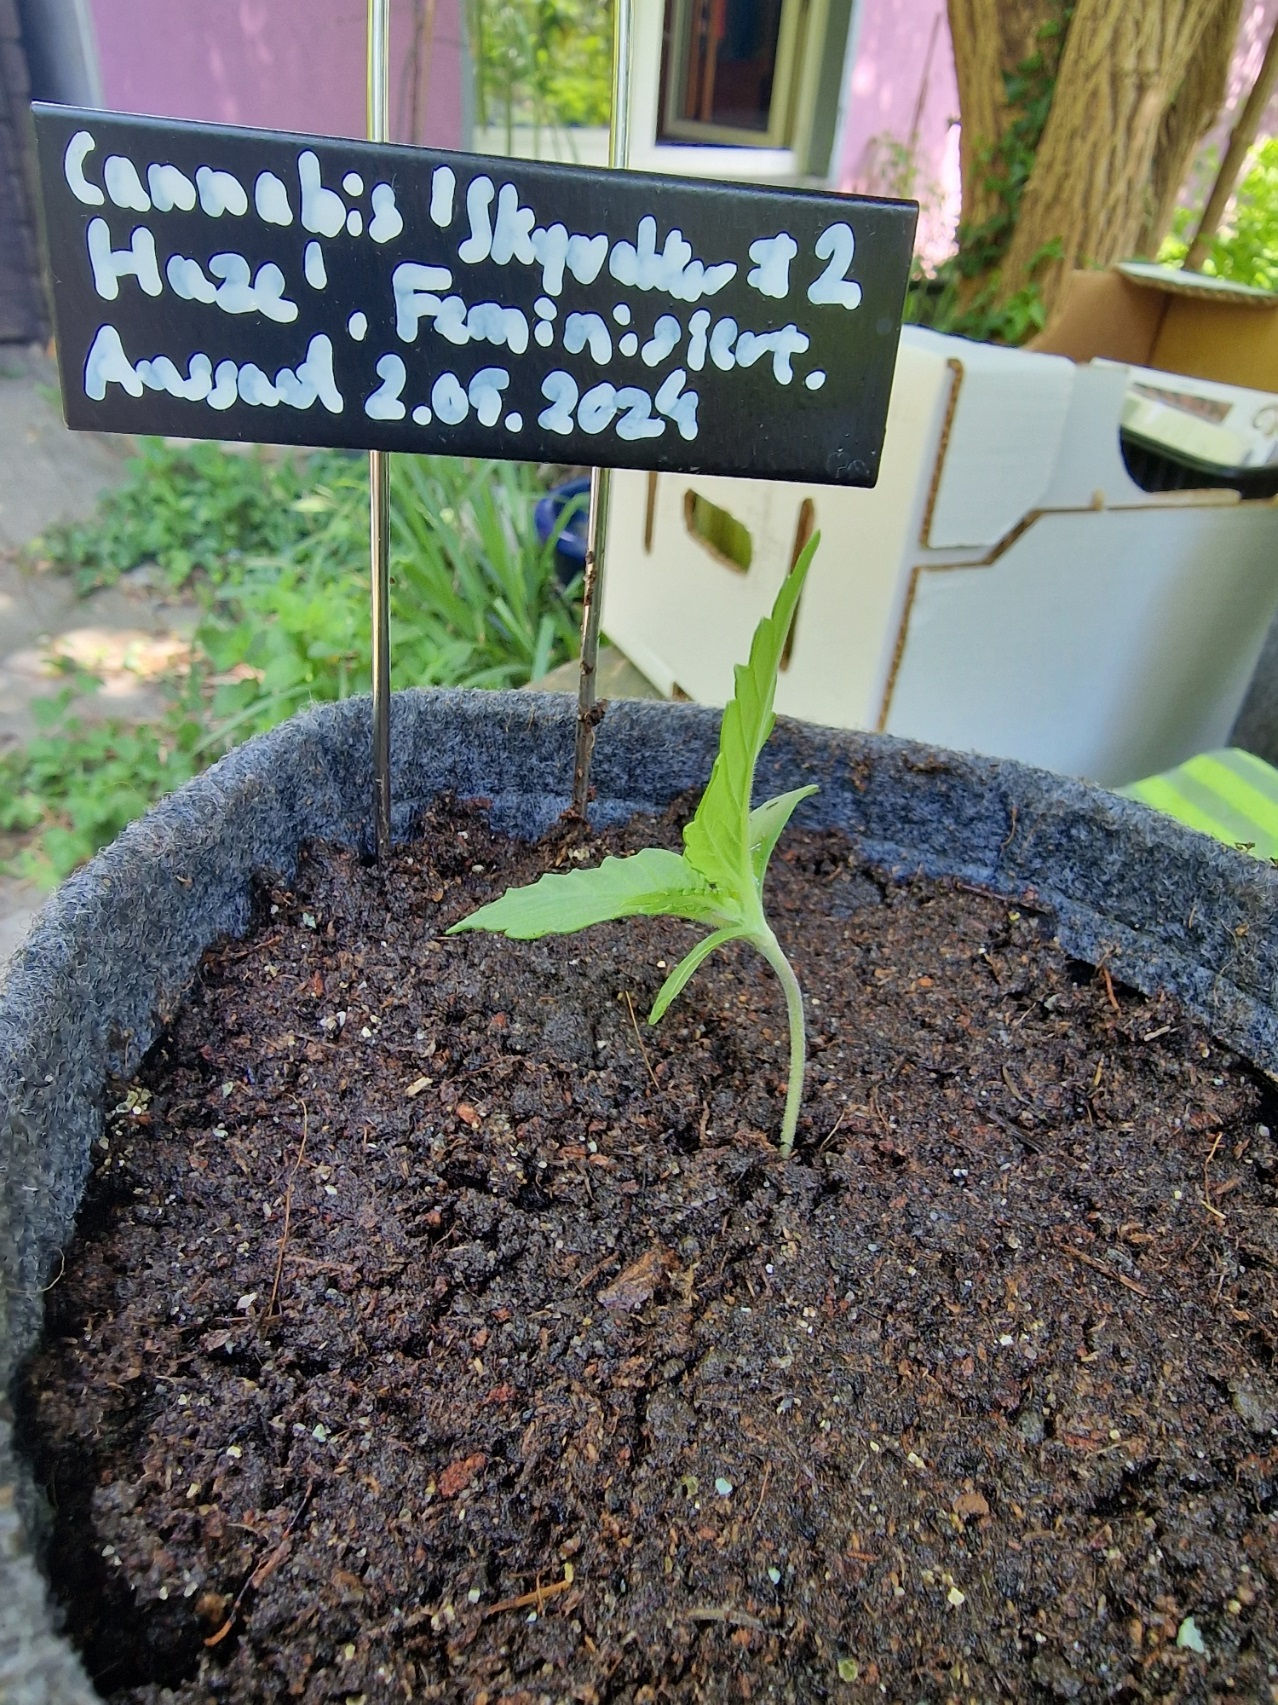
\includegraphics[width=\linewidth]{plant_02_2024-05-13}
                    \subcaption{Plant \#2}
                \end{subfigure}
                \begin{subfigure}[t]{.32\textwidth}
                    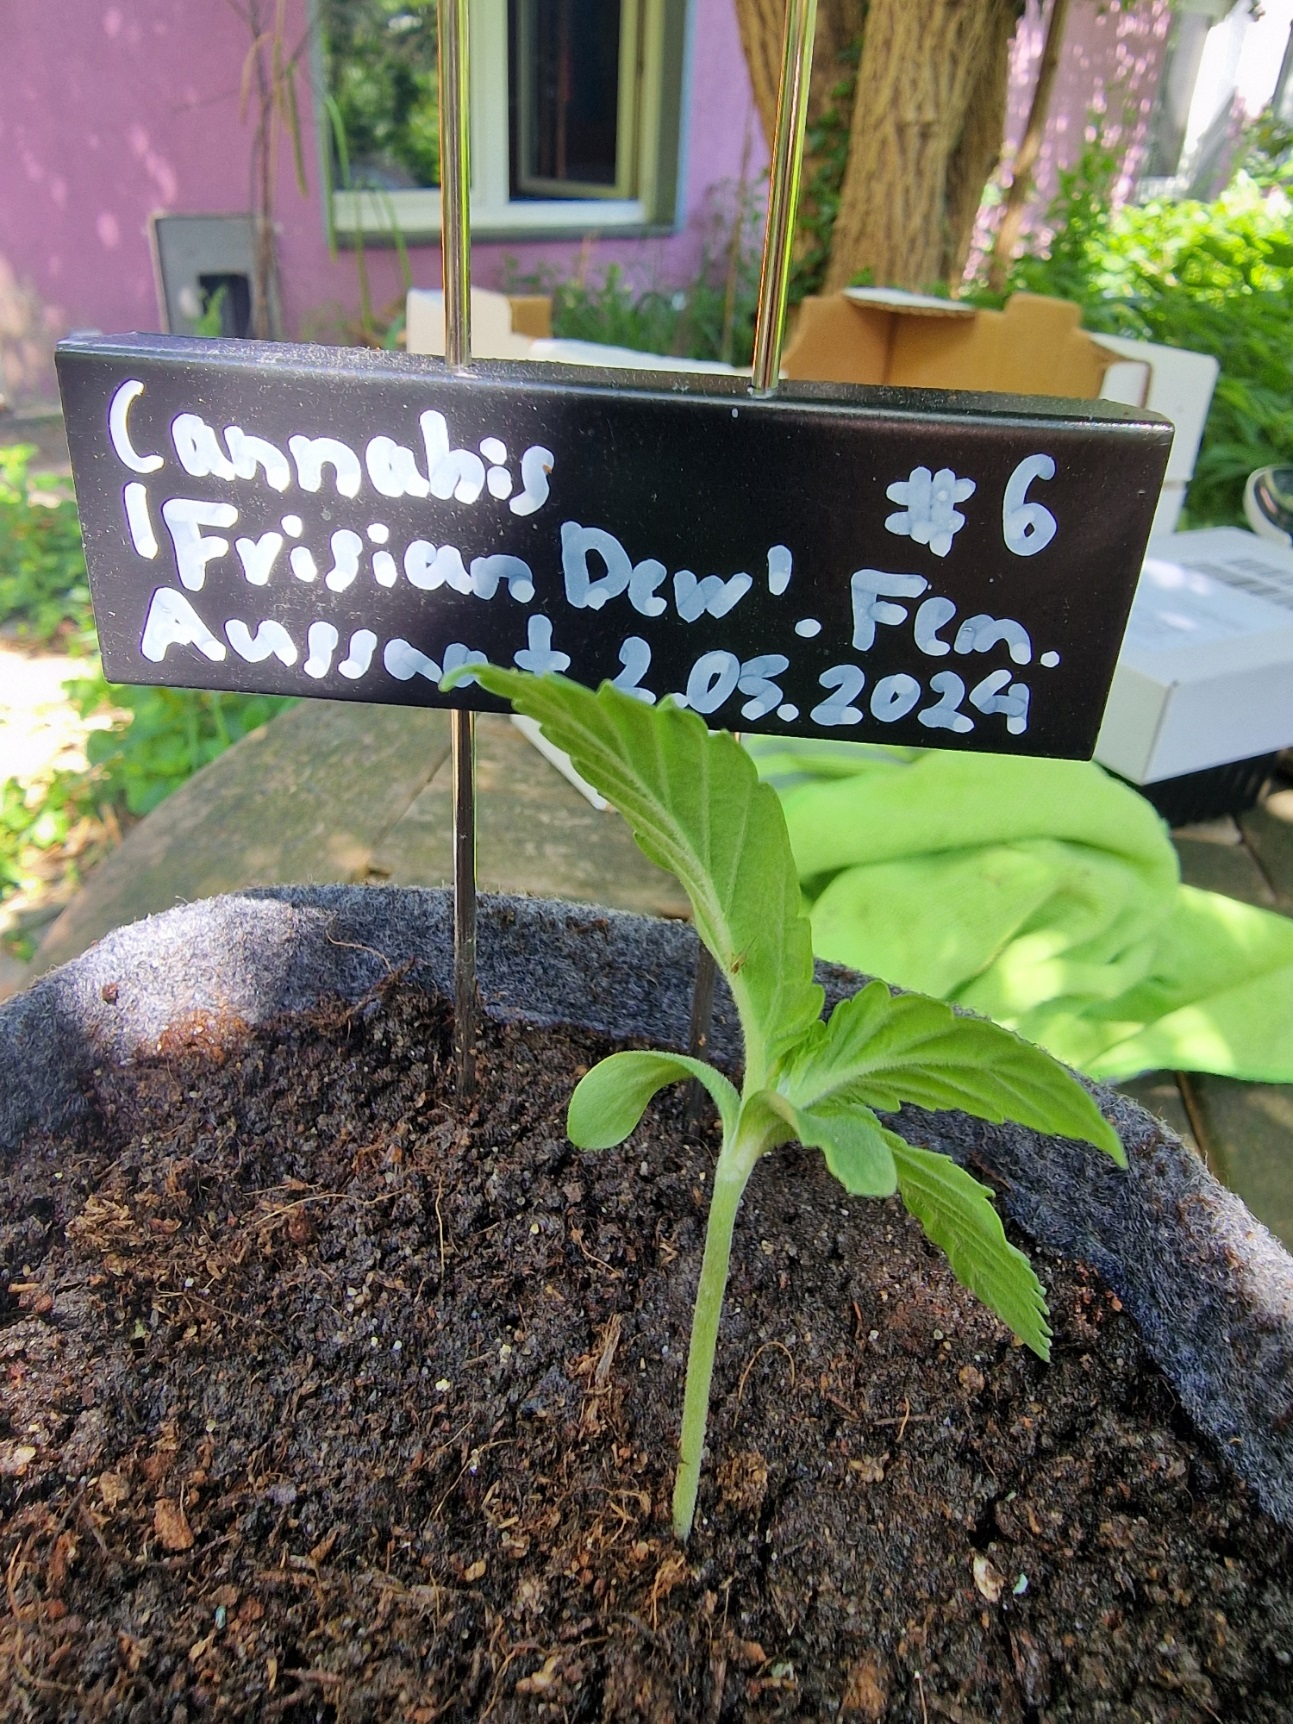
\includegraphics[width=\linewidth]{plant_06_2024-05-13}
                    \subcaption{Plant \#6}
                \end{subfigure}
                \begin{subfigure}[t]{.32\textwidth}
                    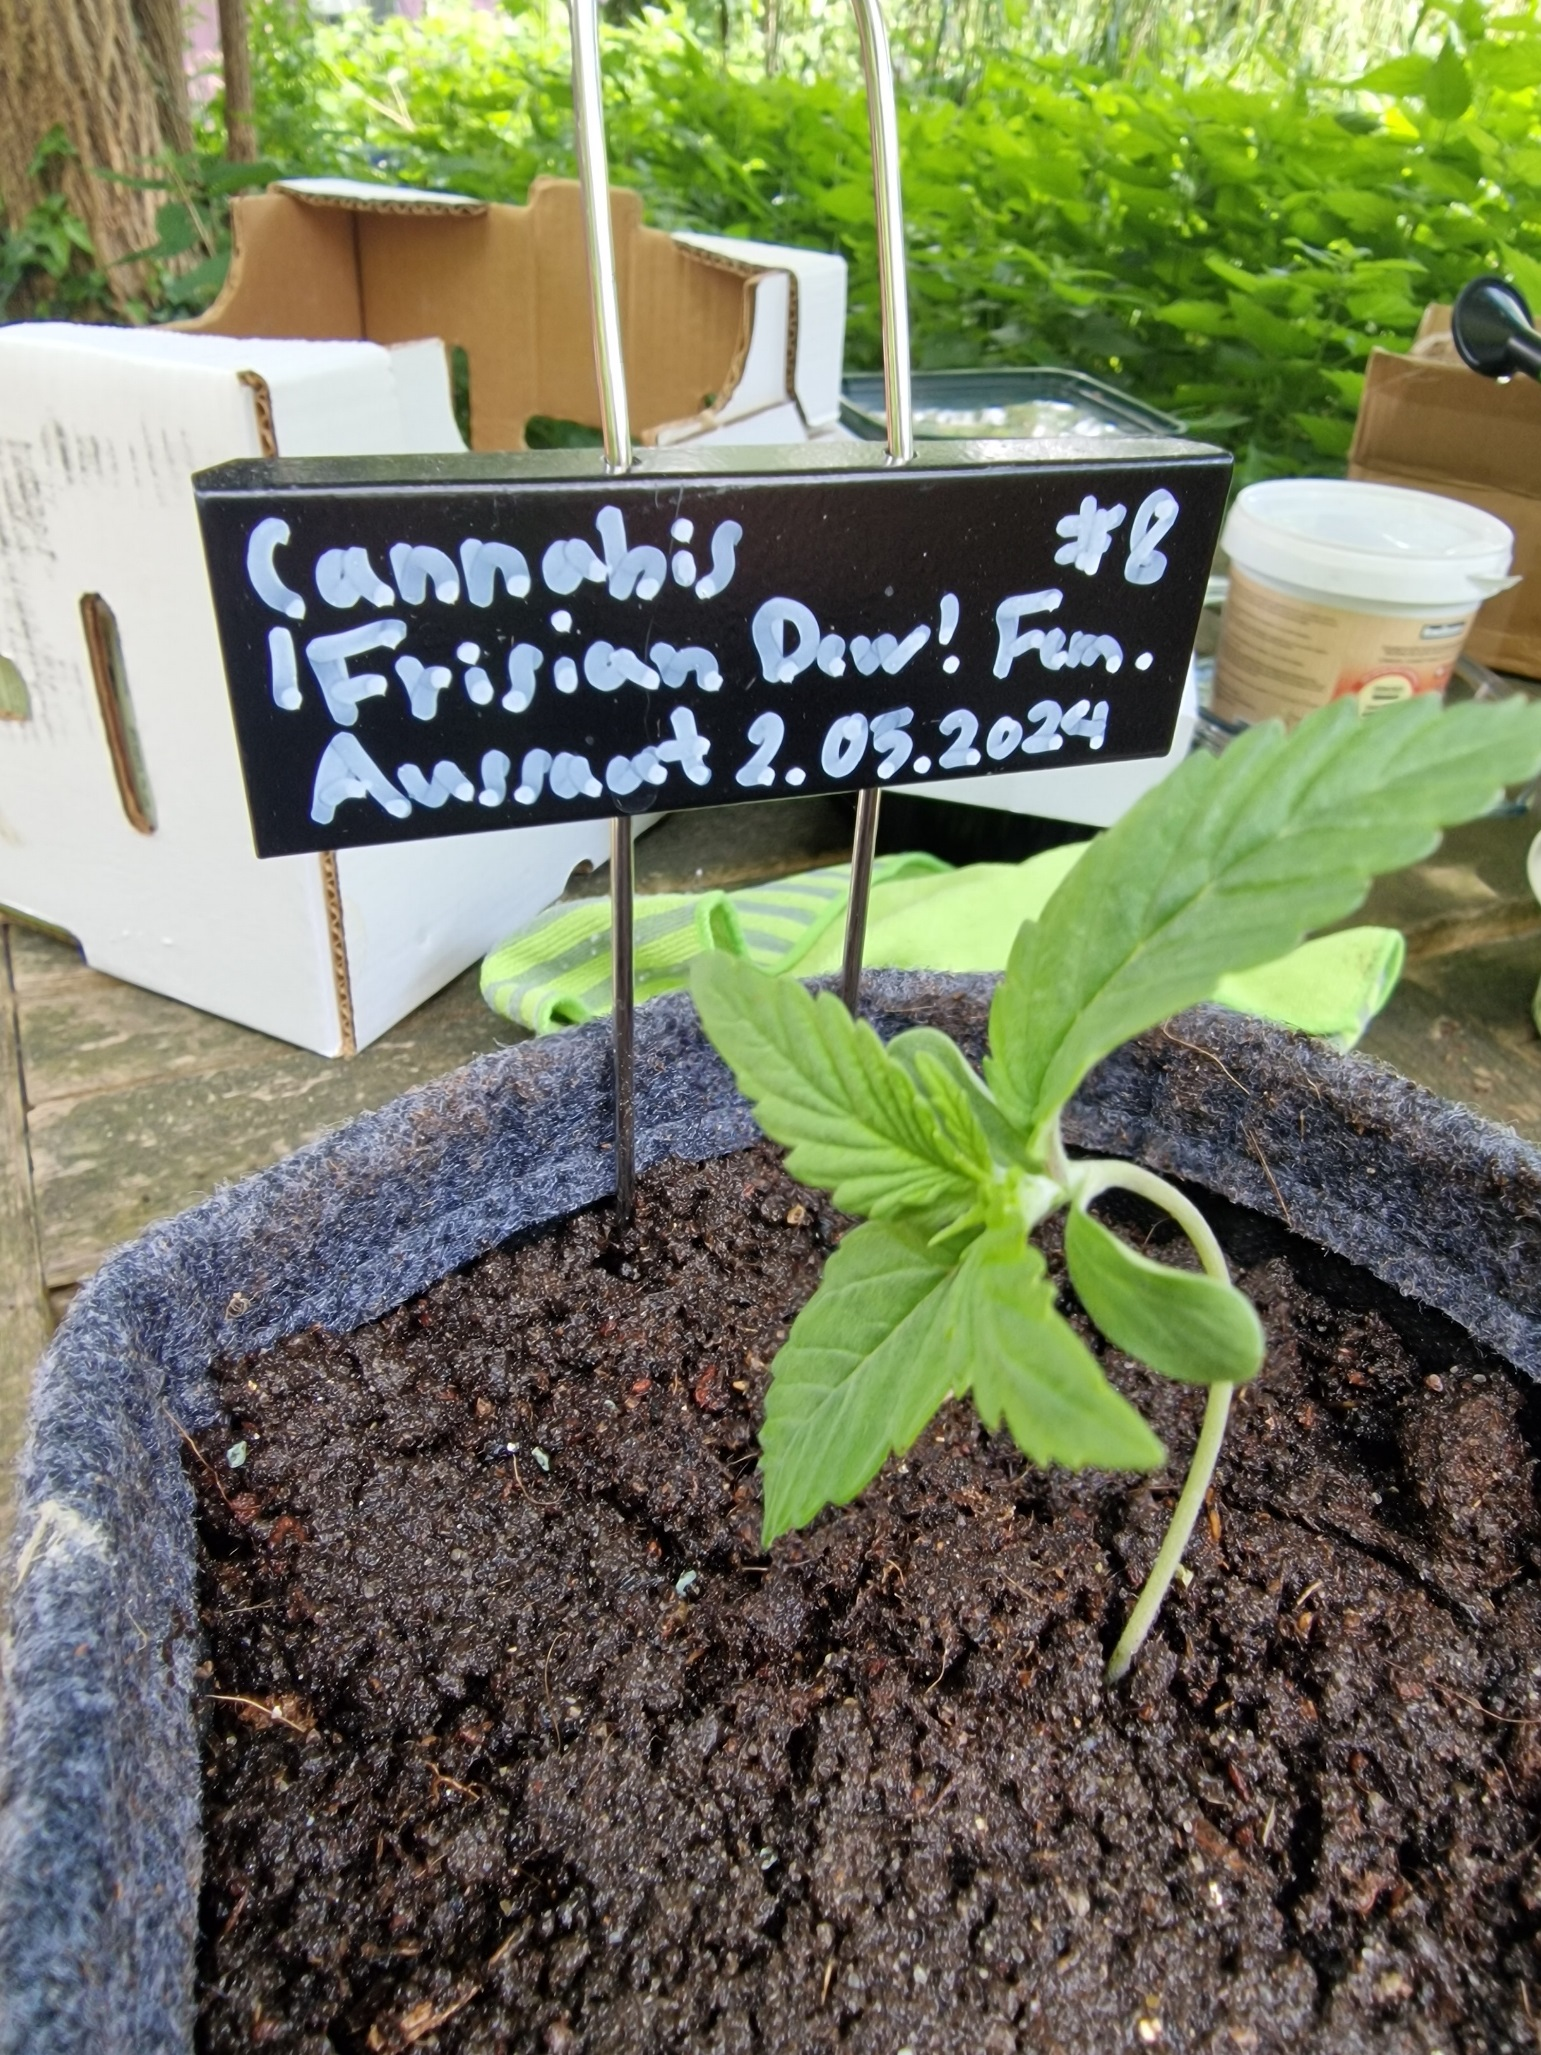
\includegraphics[width=\linewidth]{plant_08_2024-05-13}
                    \subcaption{Plant \#8}
                \end{subfigure}
                \begin{subfigure}[t]{.32\textwidth}
                    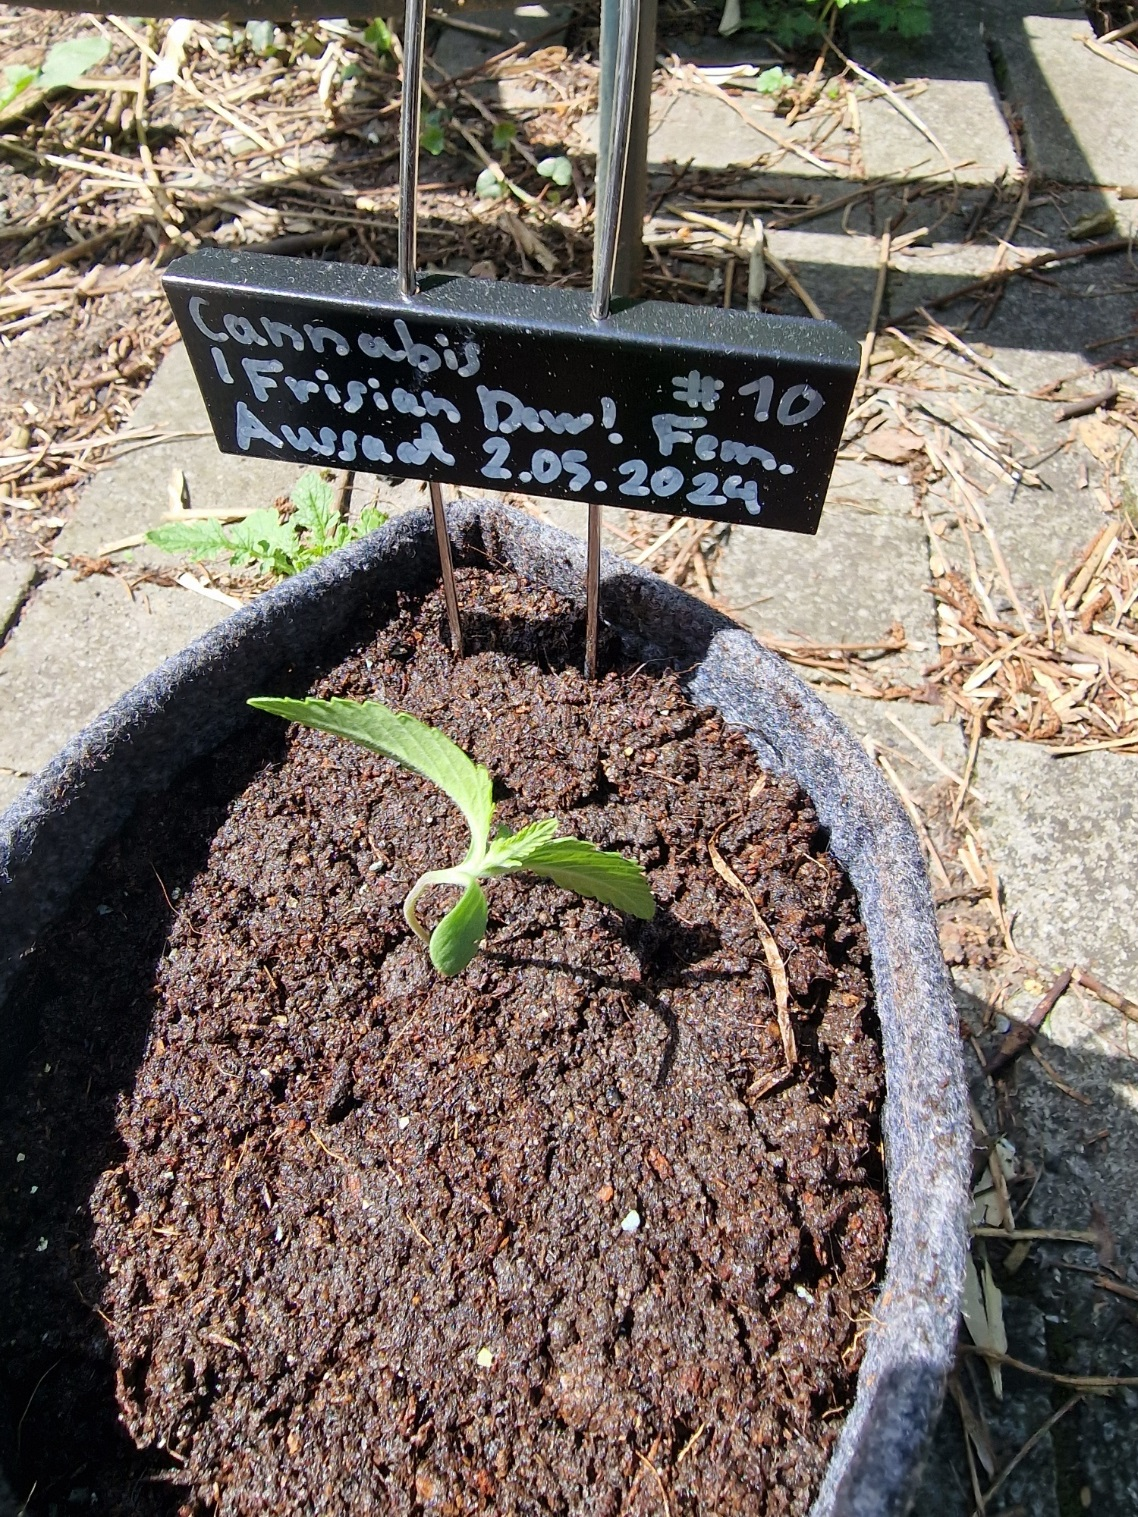
\includegraphics[width=\linewidth]{plant_10_2024-05-13}
                    \subcaption{Plant \#10}
                \end{subfigure}
                \begin{subfigure}[t]{.32\textwidth}
                    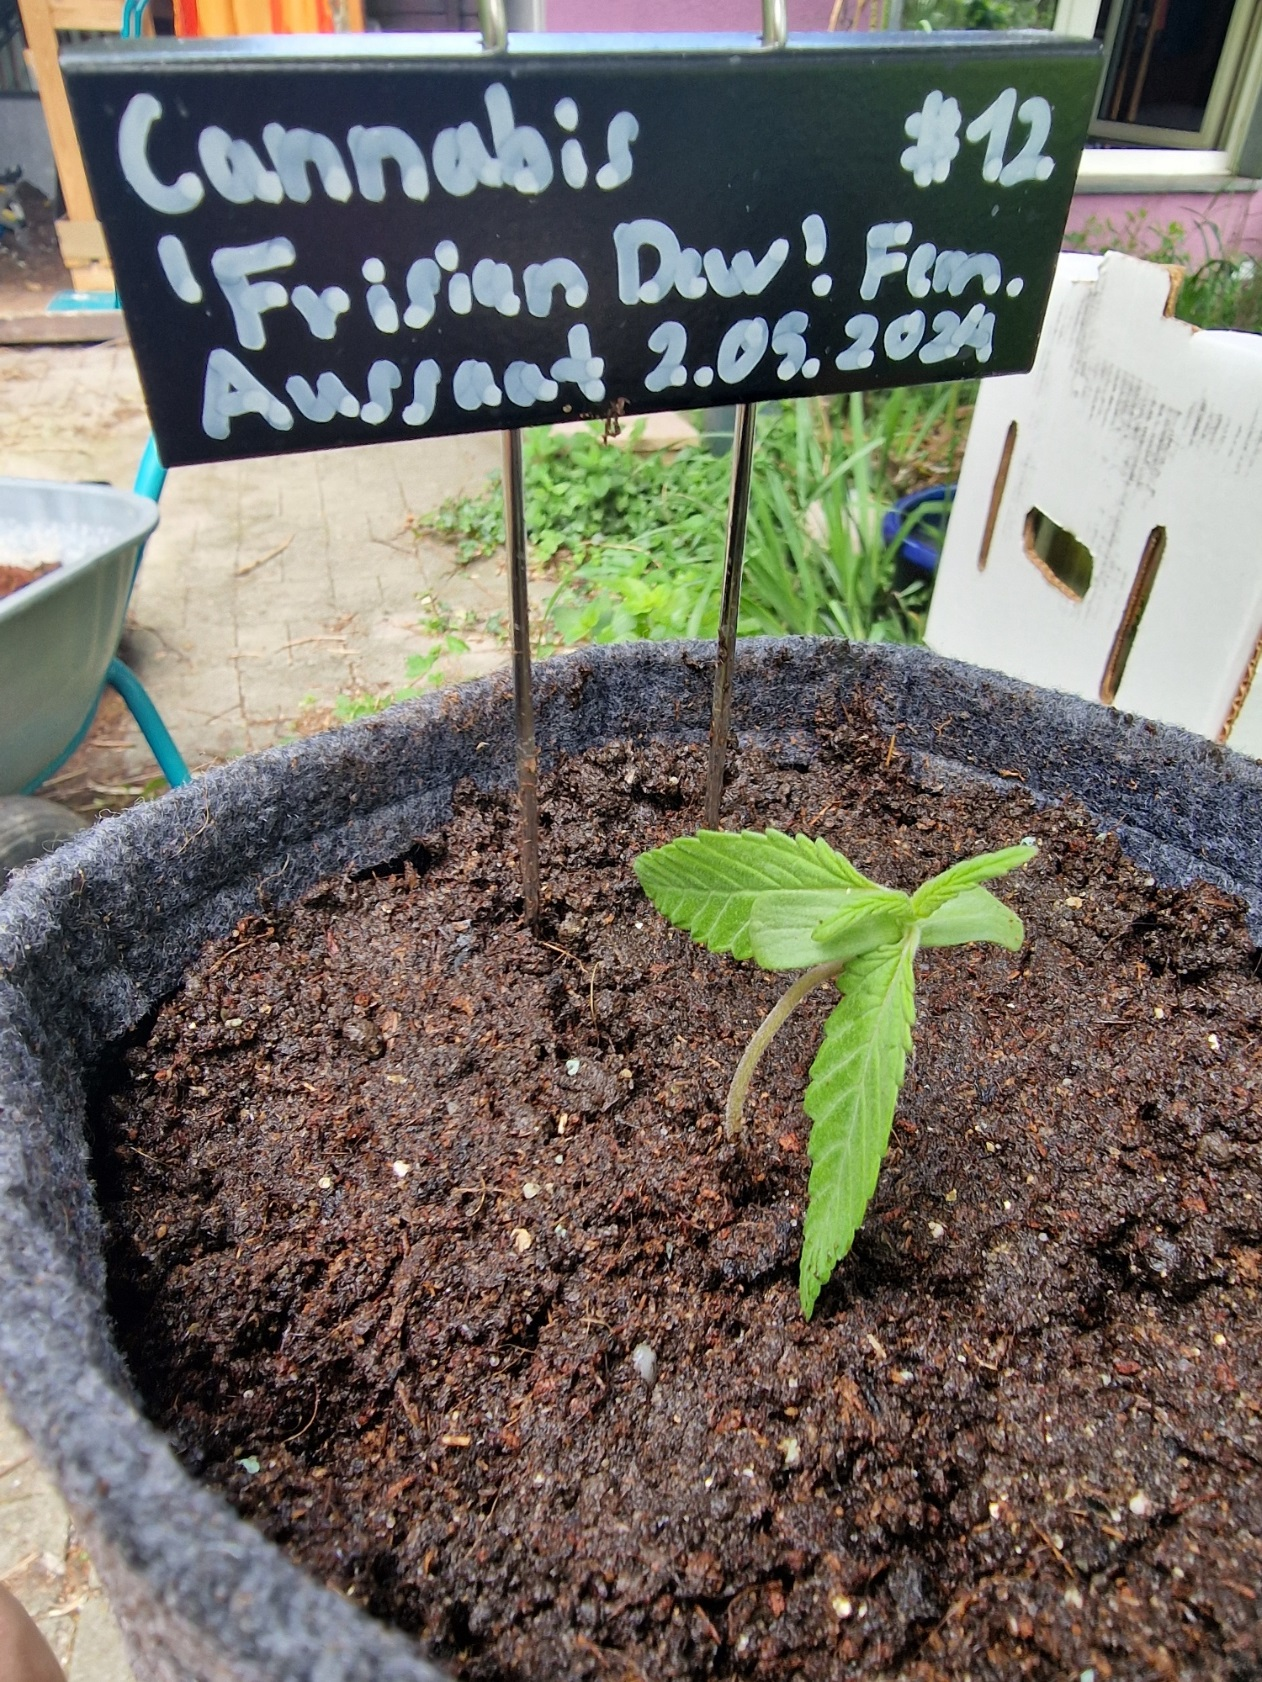
\includegraphics[width=\linewidth]{plant_12_2024-05-13}
                    \subcaption{Plant \#12}
                \end{subfigure}
                \caption{Control group}
            \end{minipage}
        \end{figure}
    \end{frame}

    \begin{frame}
        \frametitle{The plants on June 17}
        \begin{figure}[H]
            \begin{minipage}[t]{0.45\textwidth}
                \begin{subfigure}[t]{.32\textwidth}
                    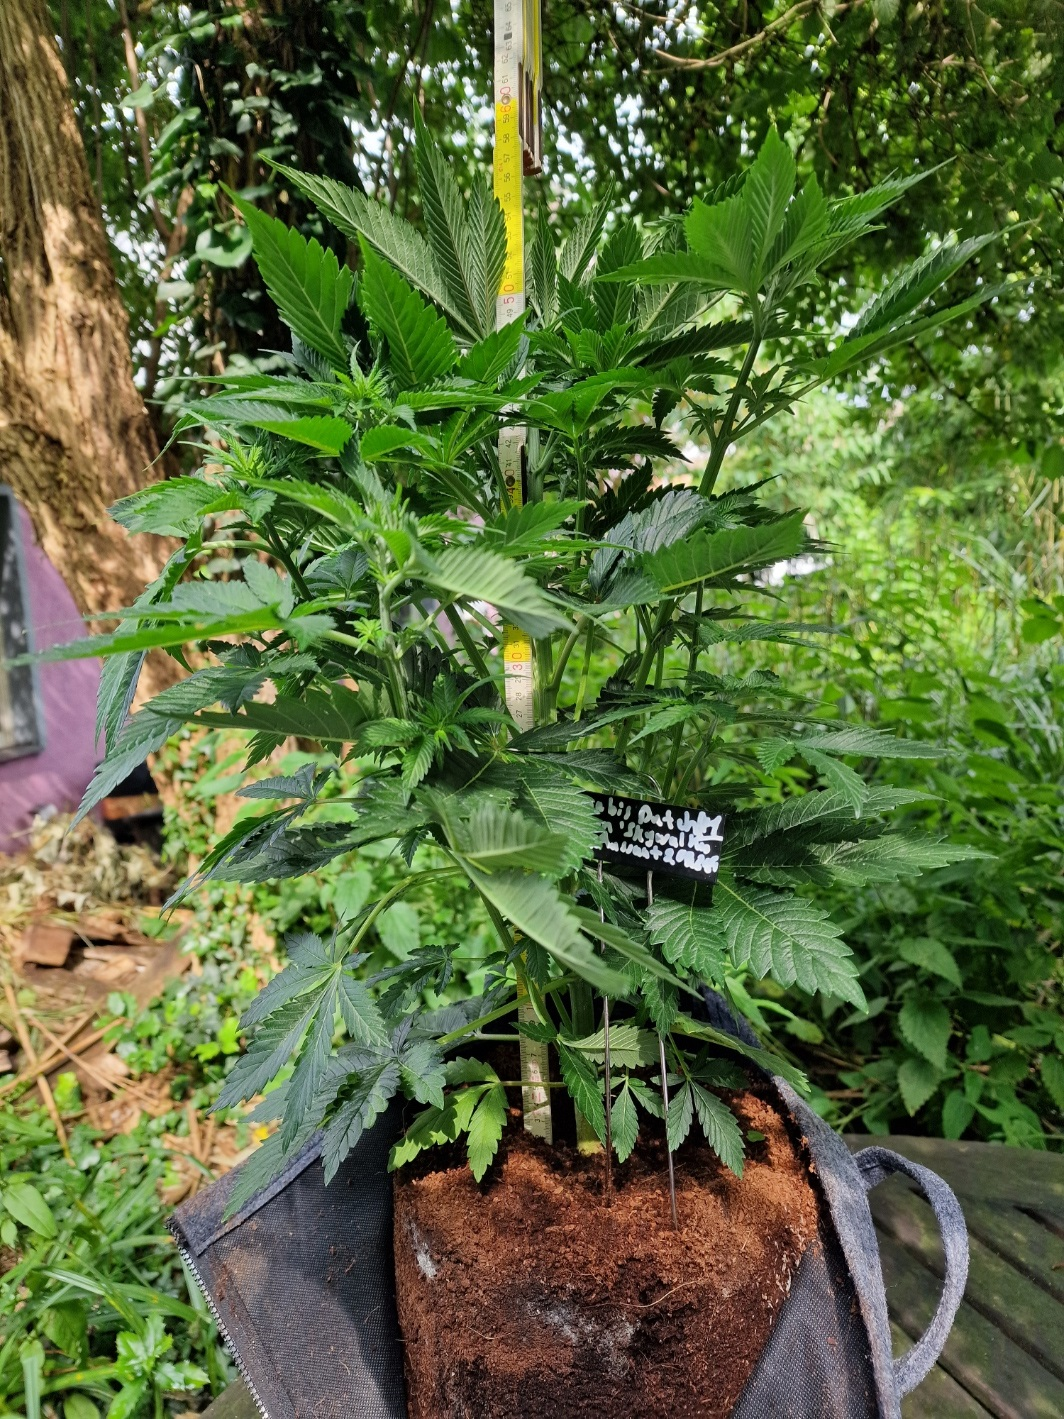
\includegraphics[width=\linewidth]{plant_01_2024-06-17}
                    \subcaption{Plant \#1}
                \end{subfigure}
                \begin{subfigure}[t]{.32\textwidth}
                    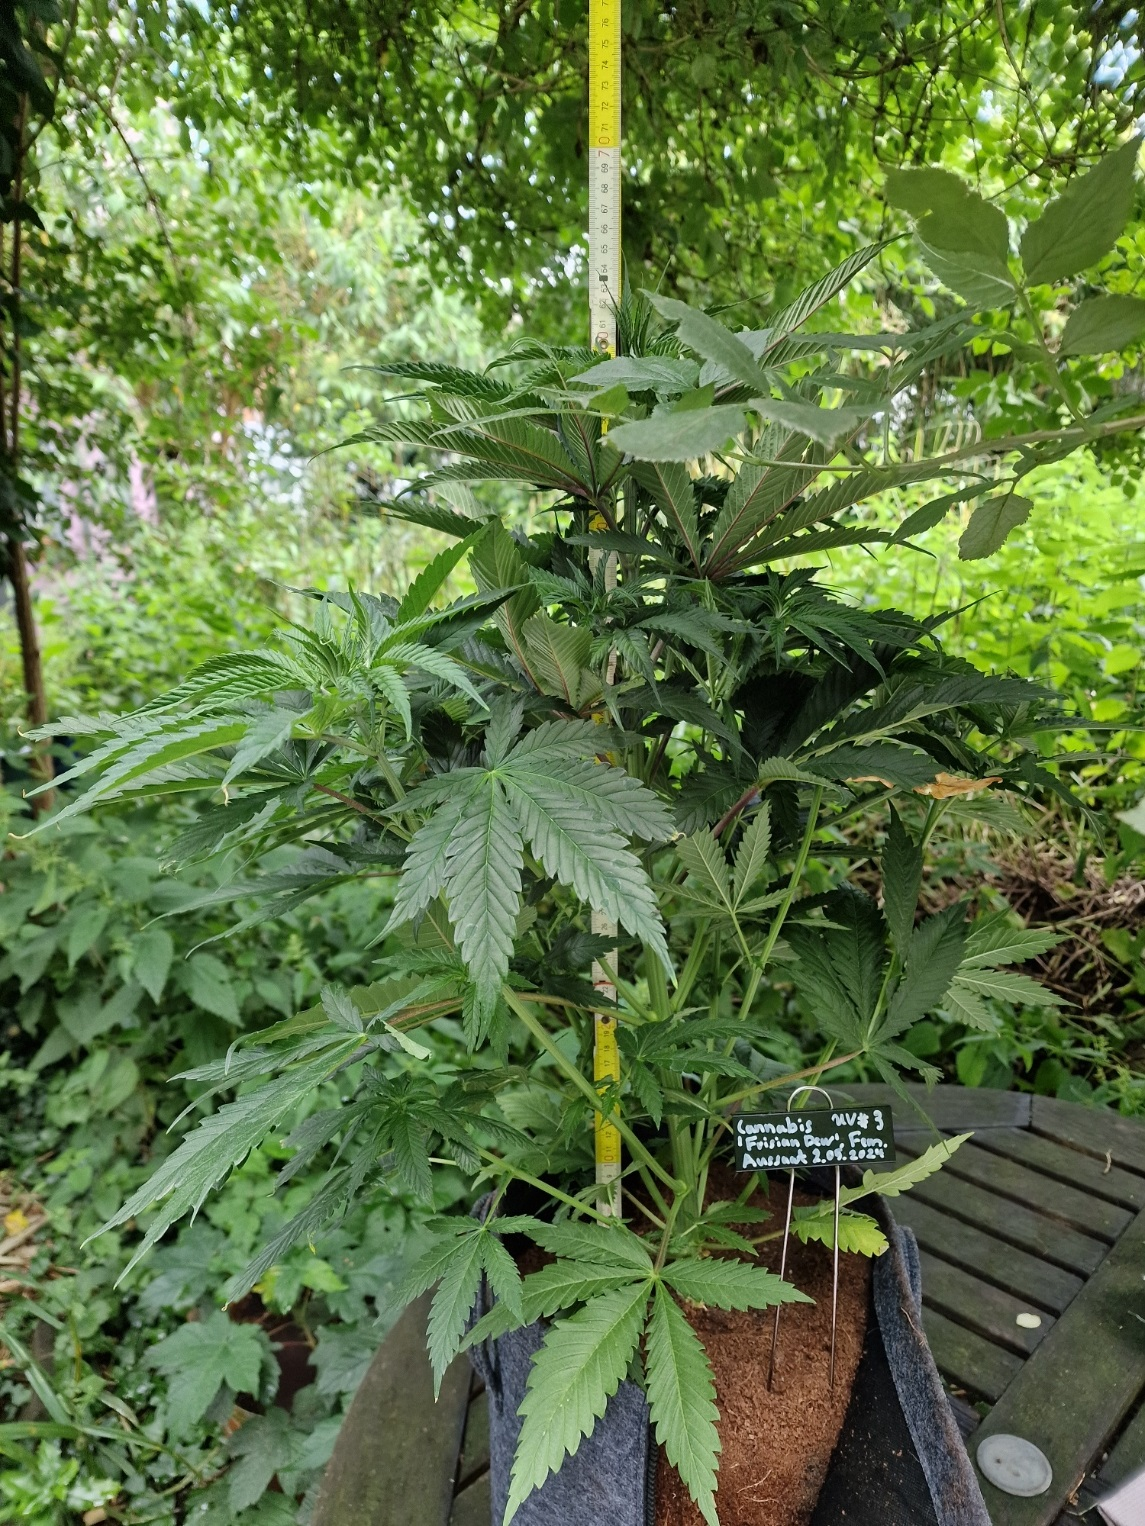
\includegraphics[width=\linewidth]{plant_03_2024-06-17}
                    \subcaption{Plant \#3}
                \end{subfigure}
                \begin{subfigure}[t]{.32\textwidth}
                    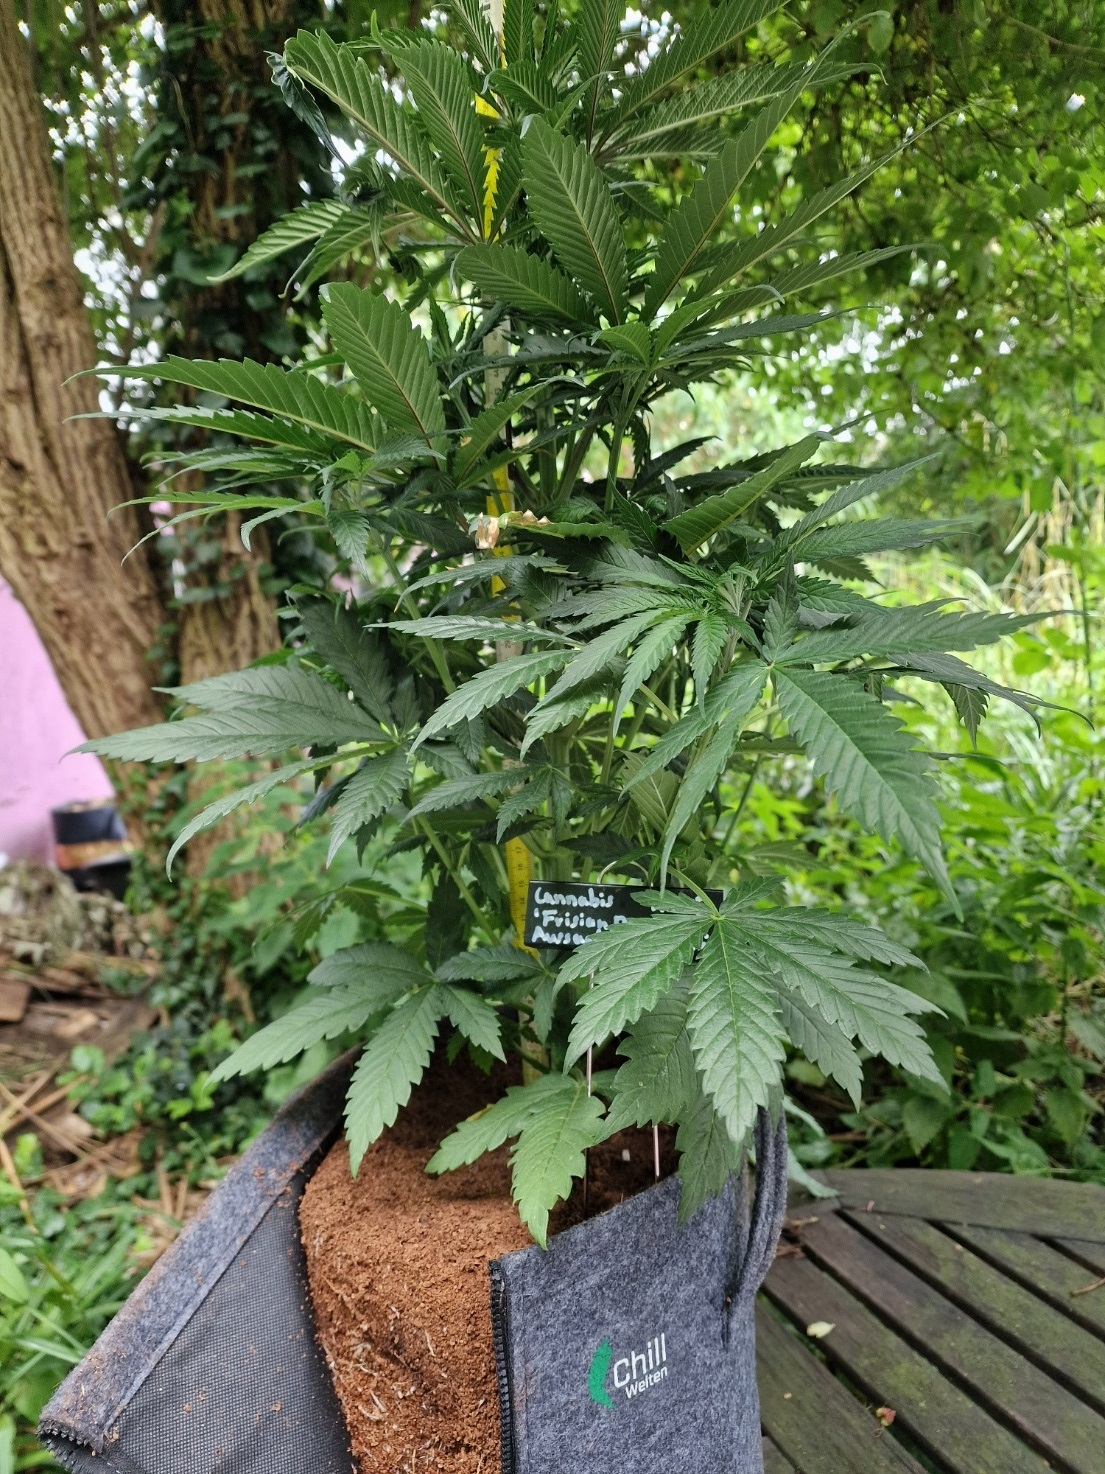
\includegraphics[width=\linewidth]{plant_05_2024-06-17}
                    \subcaption{Plant \#5}
                \end{subfigure}
                \begin{subfigure}[t]{.32\textwidth}
                    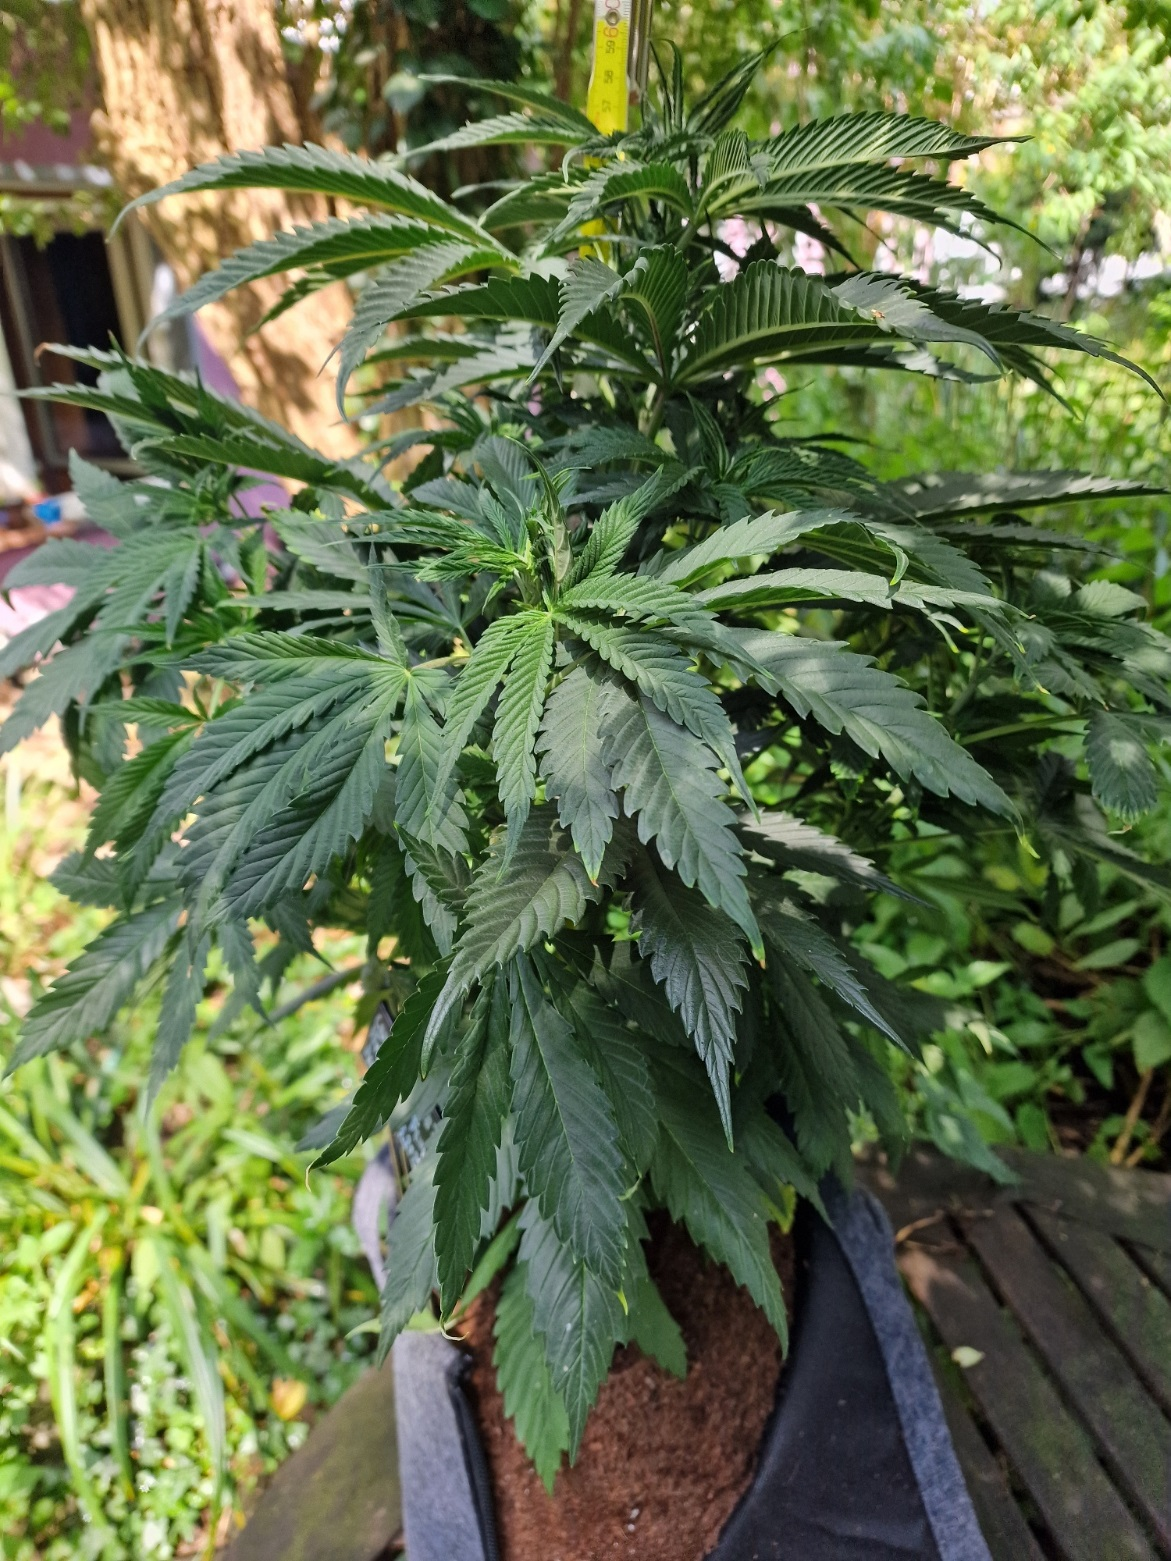
\includegraphics[width=\linewidth]{plant_07_2024-06-17}
                    \subcaption{Plant \#7}
                \end{subfigure}
                \begin{subfigure}[t]{.32\textwidth}
                    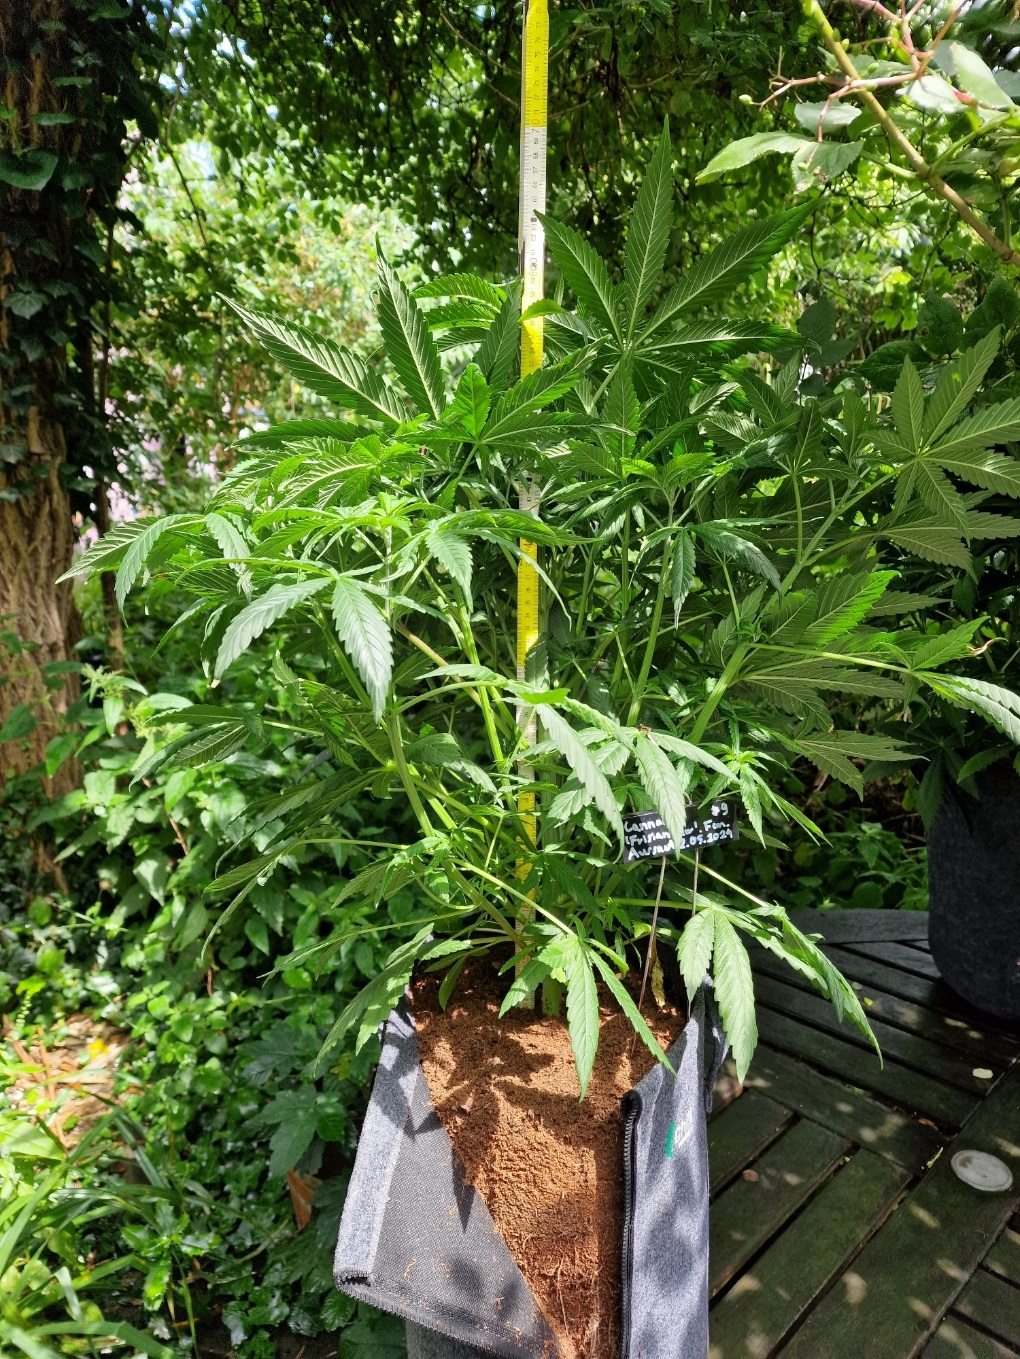
\includegraphics[width=\linewidth]{plant_09_2024-06-17}
                    \subcaption{Plant \#9}
                \end{subfigure}
                \begin{subfigure}[t]{.32\textwidth}
                    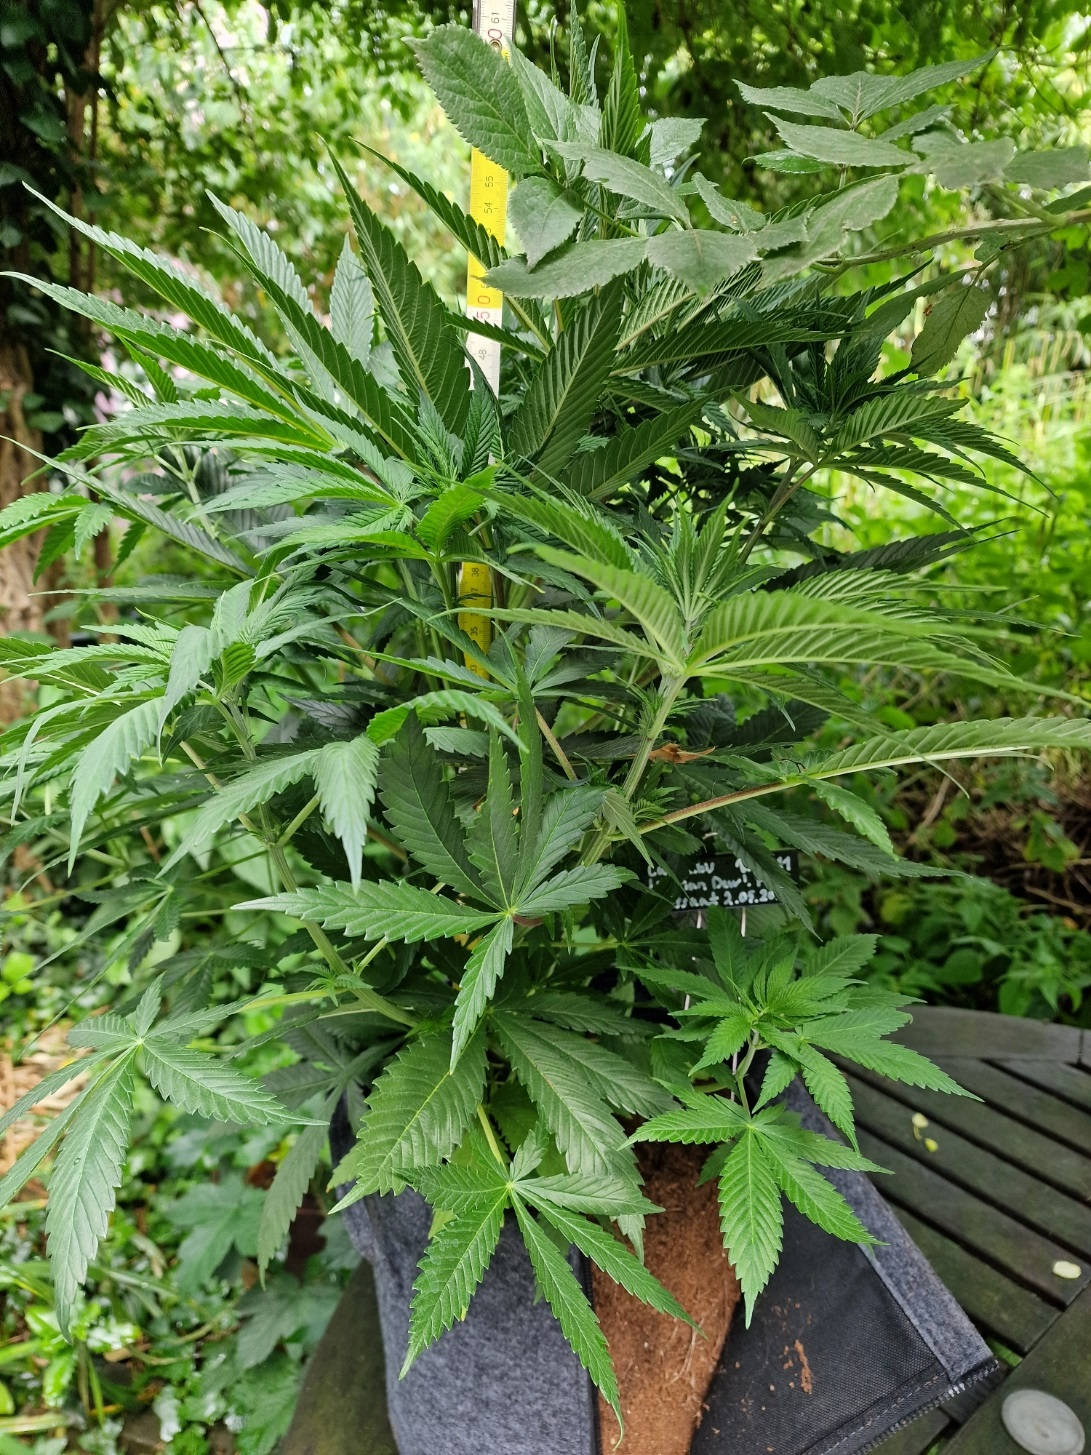
\includegraphics[width=\linewidth]{plant_11_2024-06-17}
                    \subcaption{Plant \#11}
                \end{subfigure}
                \caption{UV group}
            \end{minipage}
            \hfill
            \begin{minipage}[t]{0.45\textwidth}
                \begin{subfigure}[t]{.32\textwidth}
                    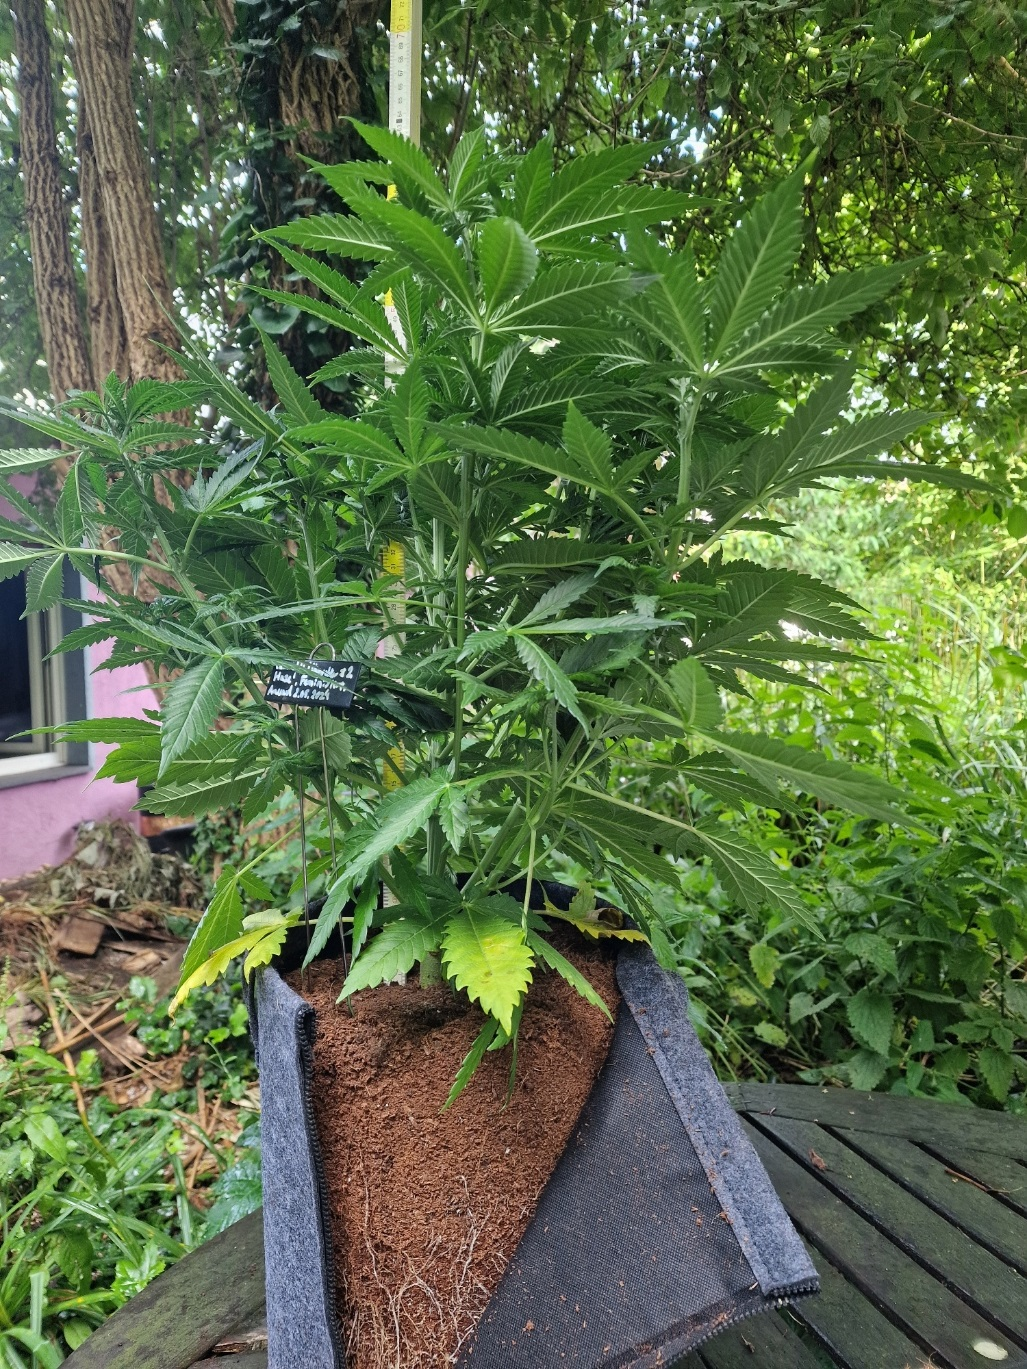
\includegraphics[width=\linewidth]{plant_02_2024-06-17}
                    \subcaption{Plant \#2}
                \end{subfigure}
                \begin{subfigure}[t]{.32\textwidth}
                    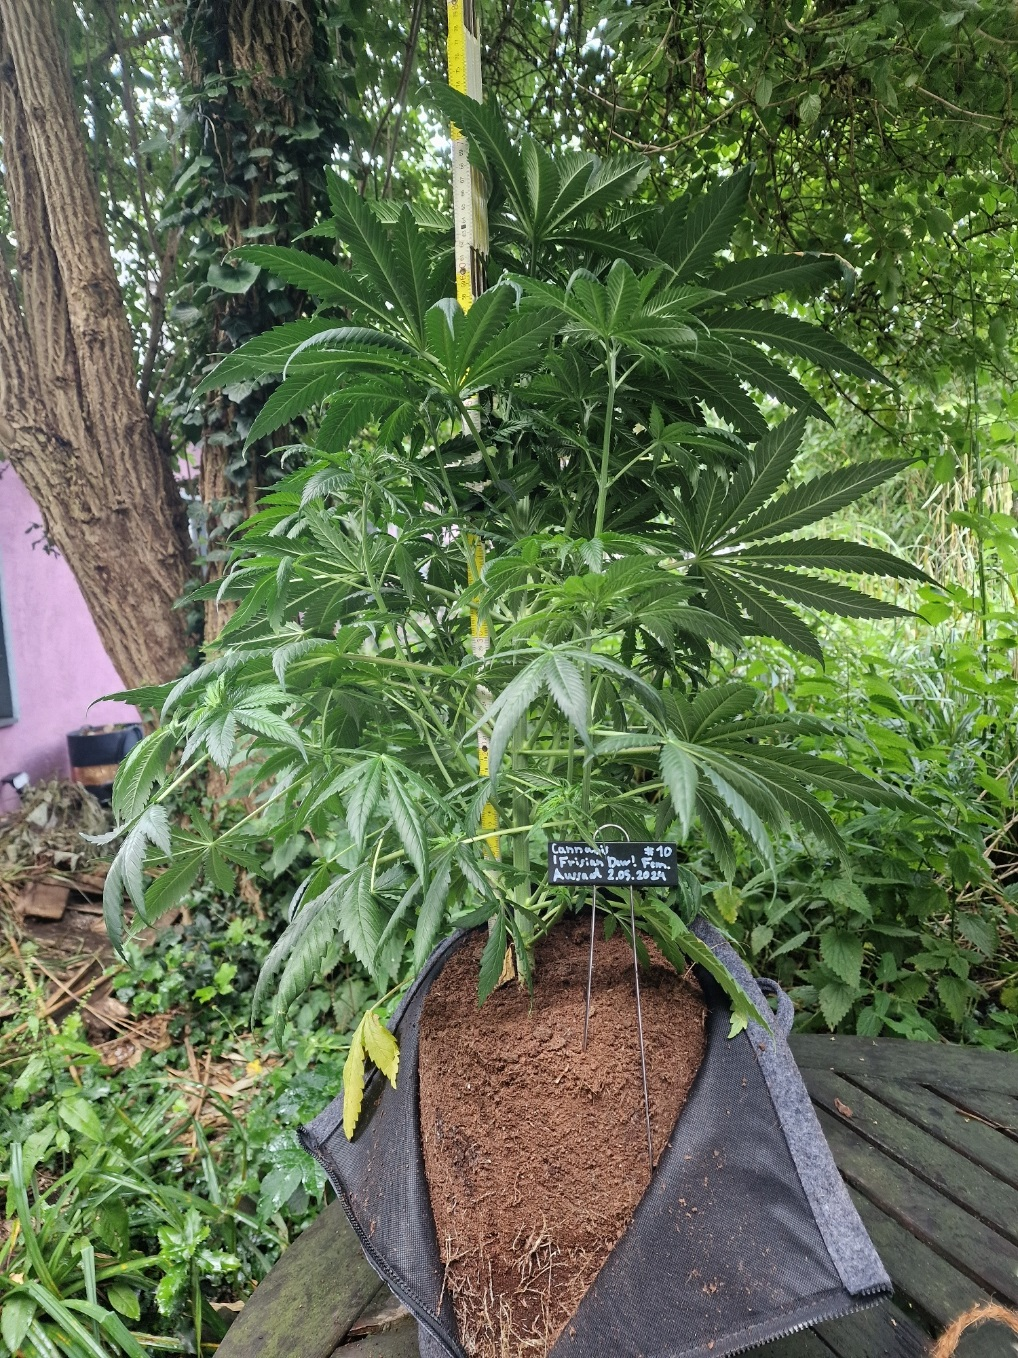
\includegraphics[width=\linewidth]{plant_06_2024-06-17}
                    \subcaption{Plant \#6}
                \end{subfigure}
                \begin{subfigure}[t]{.32\textwidth}
                    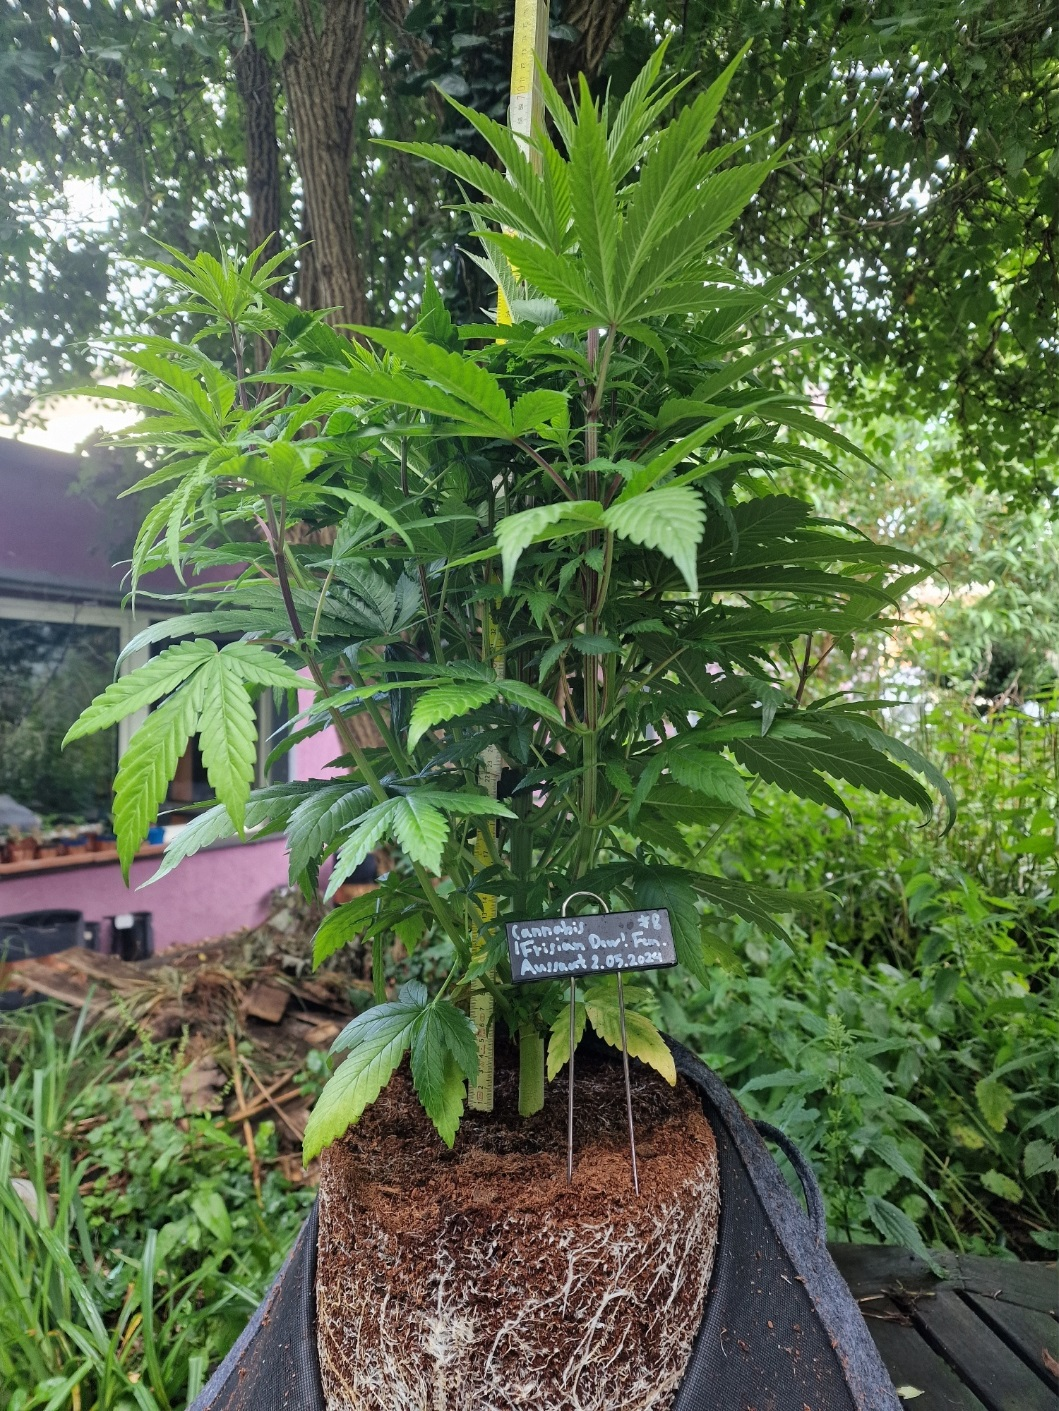
\includegraphics[width=\linewidth]{plant_08_2024-06-17}
                    \subcaption{Plant \#8}
                \end{subfigure}
                \begin{subfigure}[t]{.32\textwidth}
                    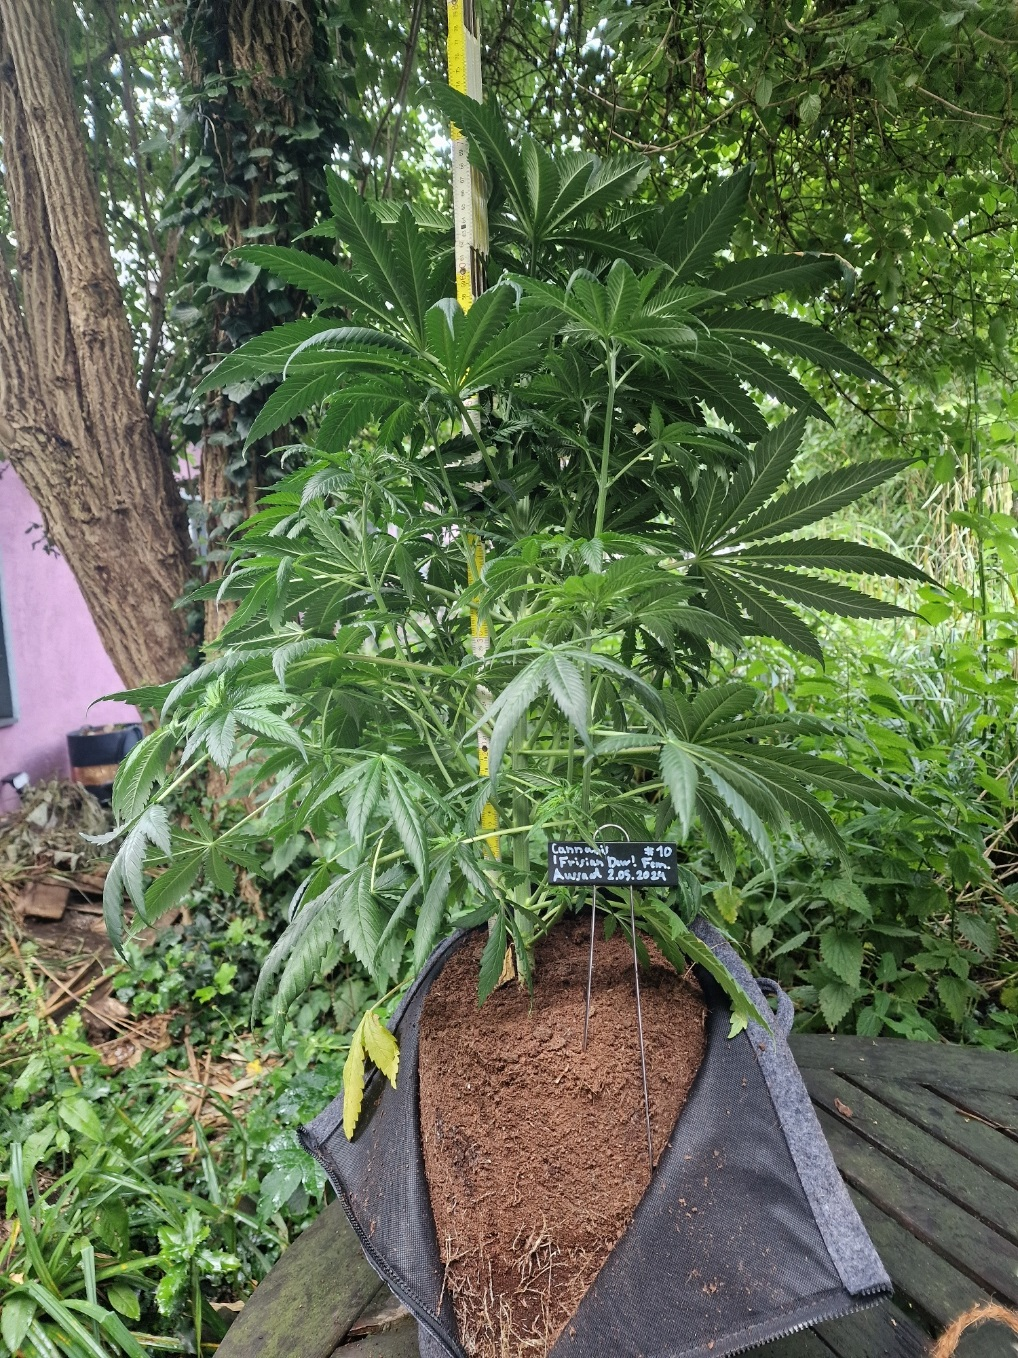
\includegraphics[width=\linewidth]{plant_10_2024-06-17}
                    \subcaption{Plant \#10}
                \end{subfigure}
                \begin{subfigure}[t]{.32\textwidth}
                    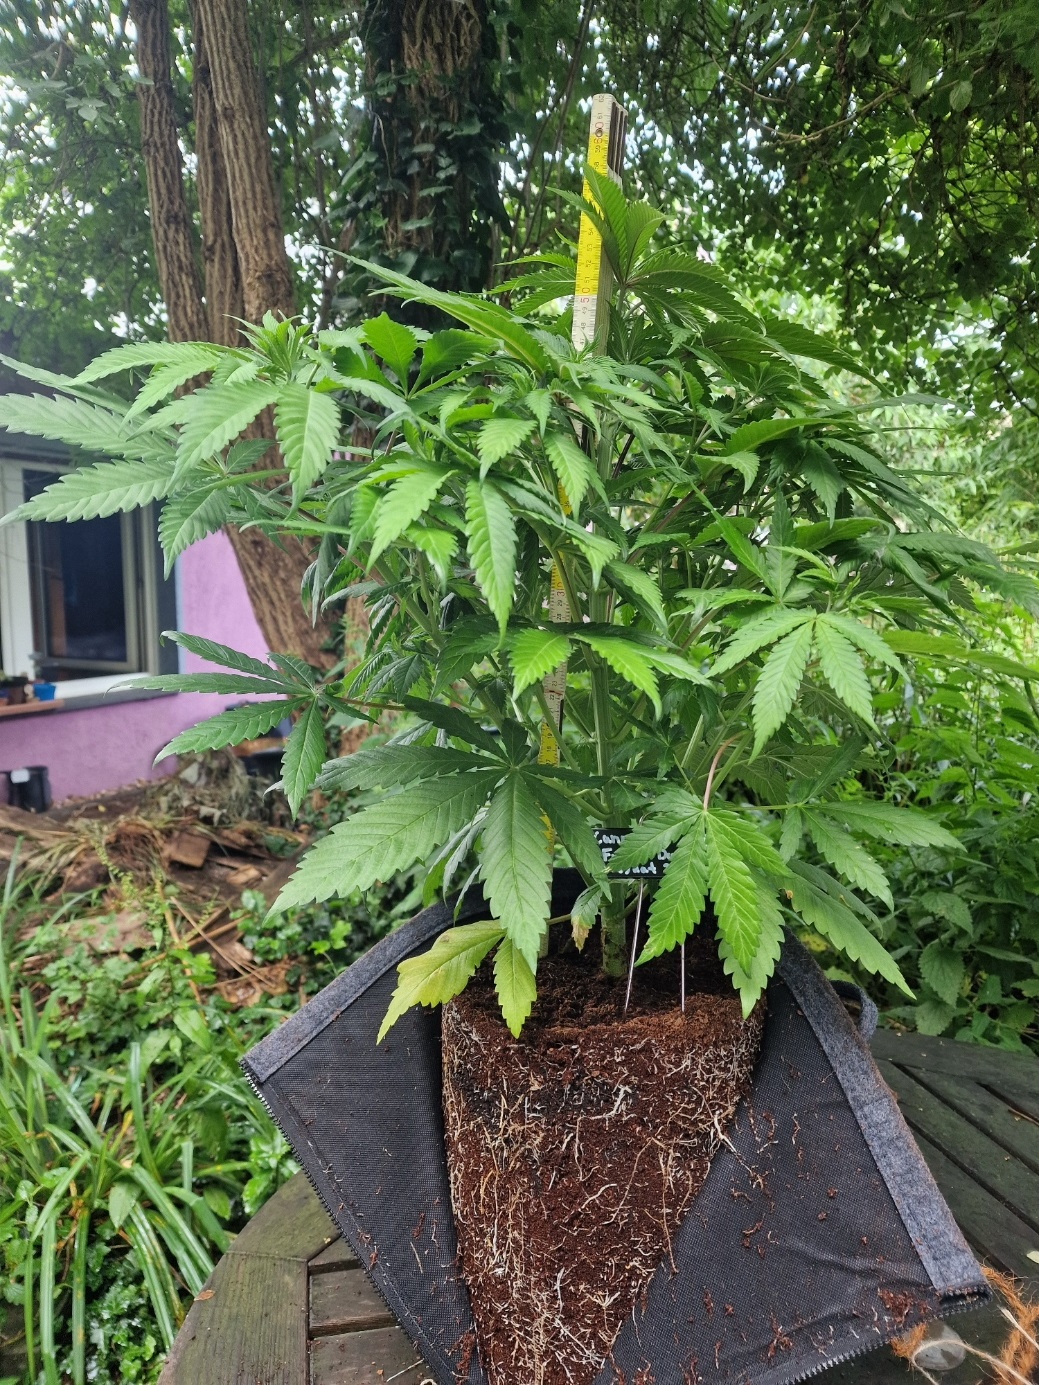
\includegraphics[width=\linewidth]{plant_12_2024-06-17}
                    \subcaption{Plant \#12}
                \end{subfigure}
                \caption{Control group}
            \end{minipage}
        \end{figure}
    \end{frame}

    \begin{frame}
        \frametitle{The plants on June 17}
        \begin{figure}[H]
            \begin{minipage}[t]{0.45\textwidth}
                \begin{subfigure}[t]{0.99\textwidth}
                    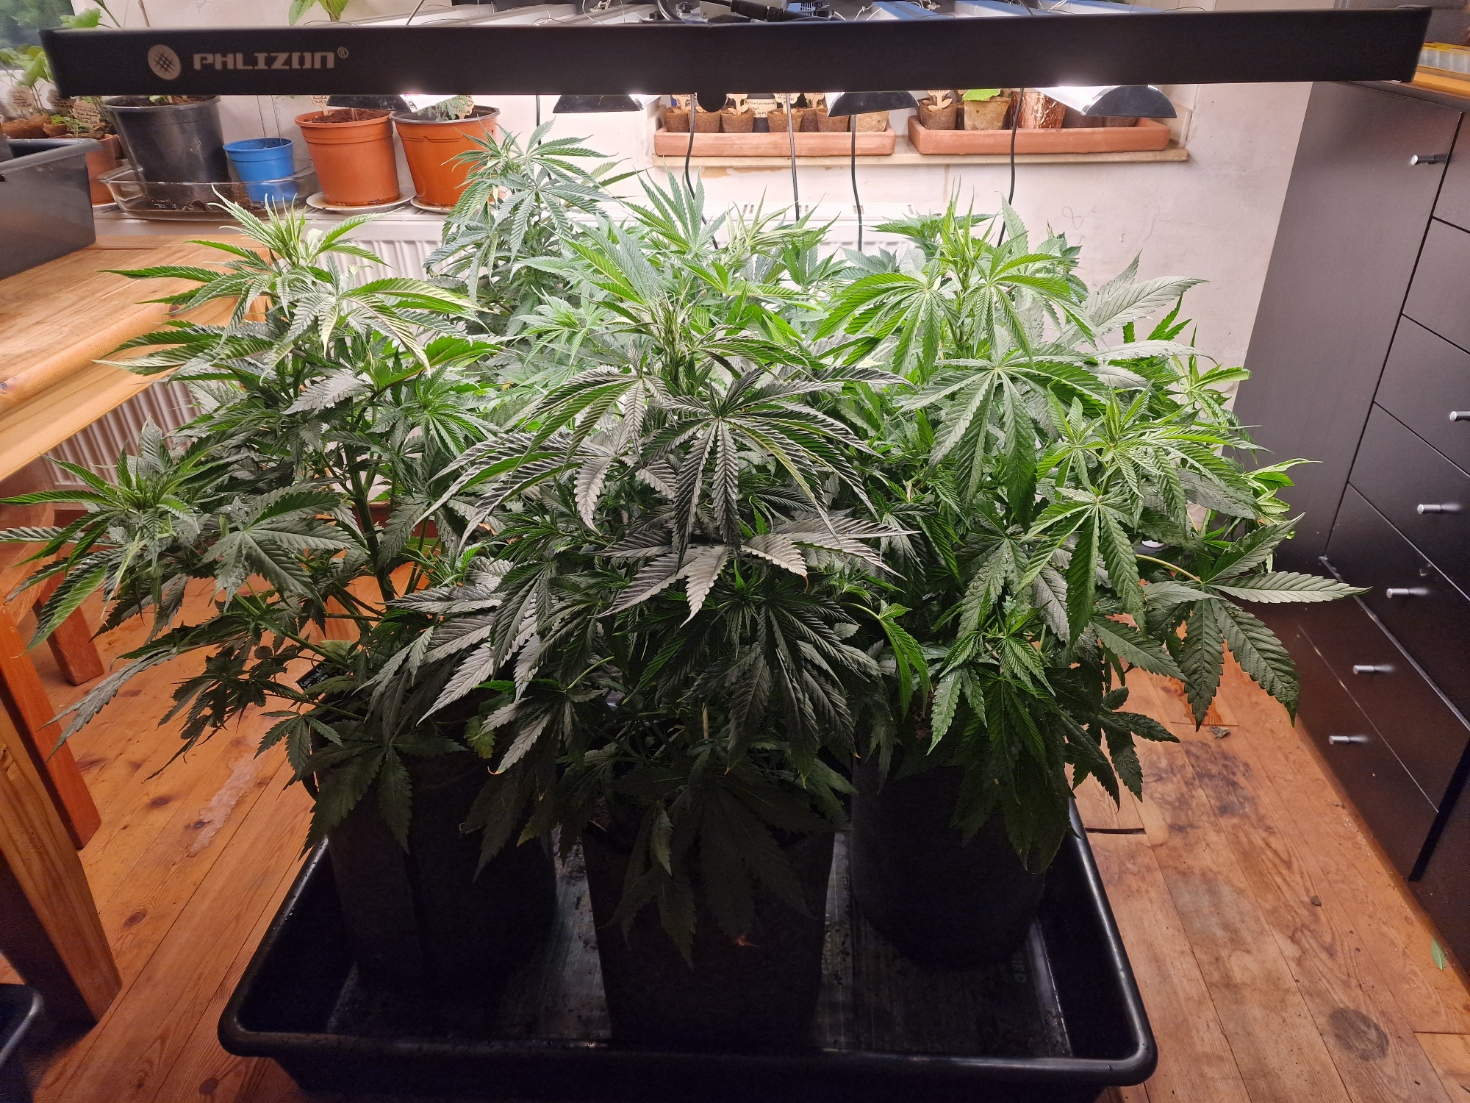
\includegraphics[width=\linewidth]{plant_uv_2024-06-17}
                \end{subfigure}
                \caption{UV group}
            \end{minipage}
            \hfill
            \begin{minipage}[t]{0.45\textwidth}
                \begin{subfigure}[t]{0.99\textwidth}
                    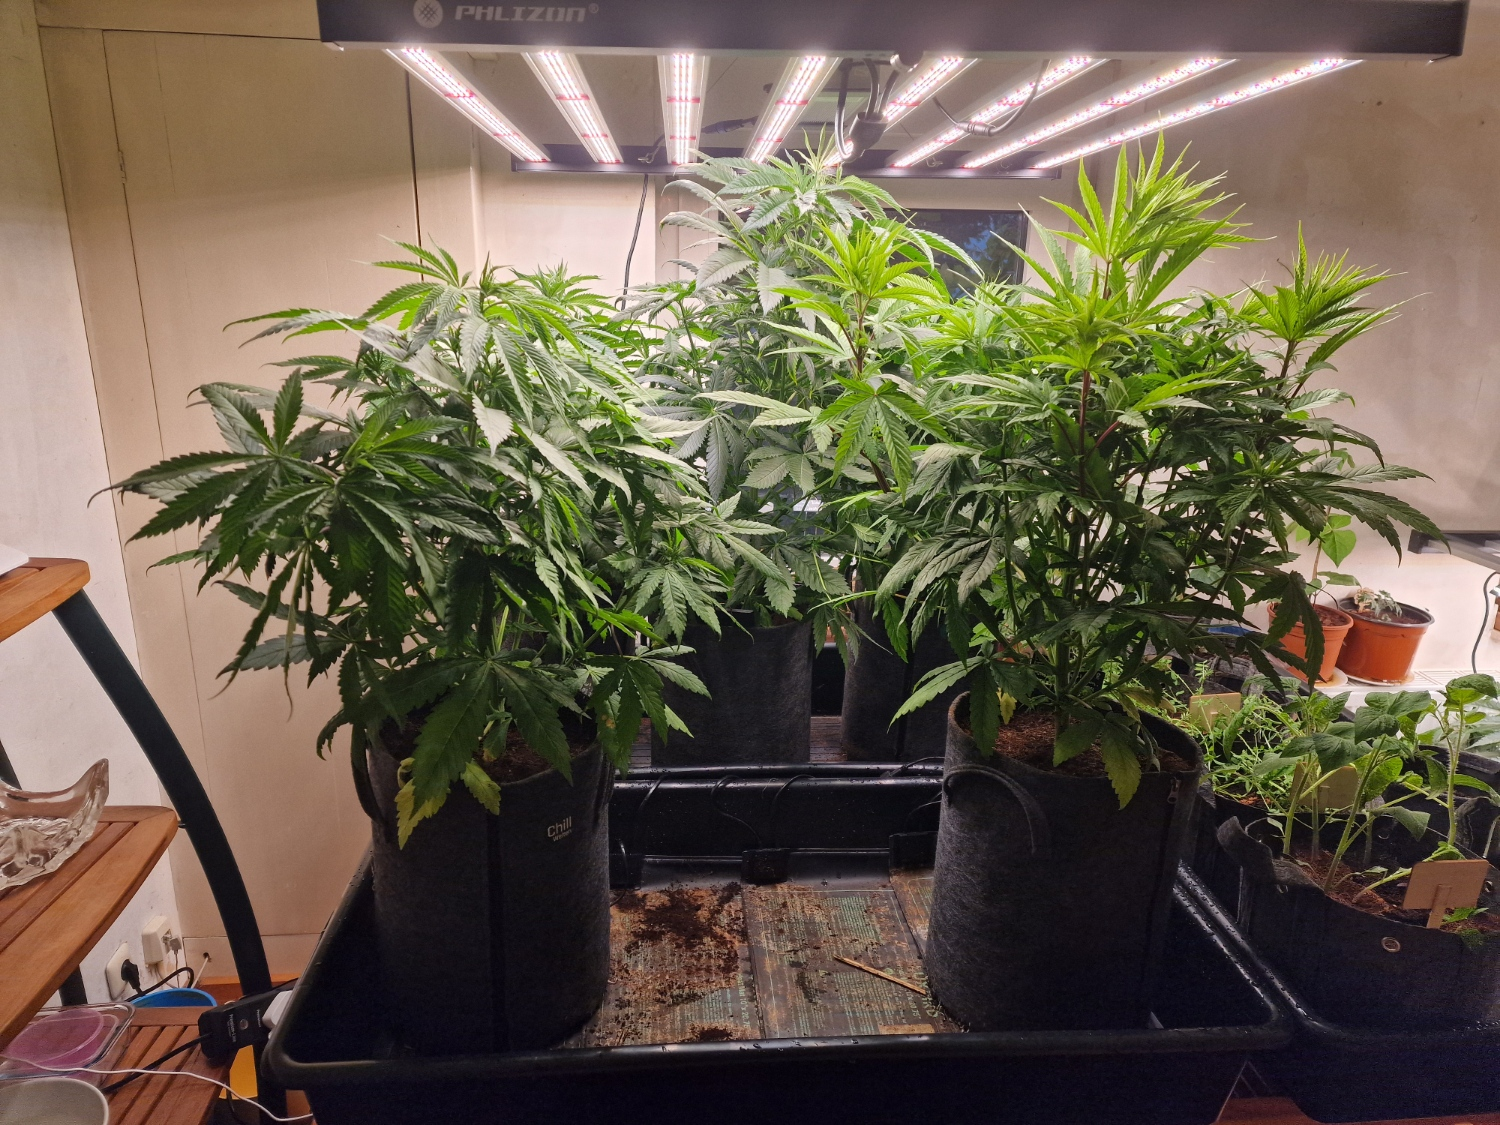
\includegraphics[width=\linewidth]{plant_ctrl_2024-06-17}
                \end{subfigure}
                \caption{Control group}
            \end{minipage}
        \end{figure}
    \end{frame}

    \begin{frame}
        \frametitle{Measured growth parameters}
        \footnotesize
        \begin{table}
            \begin{tabular}{llcccc}
                \hline
                \hline
                \textbf{Group} & \textbf{Cultivar} & \textbf{Plant \#} & \textbf{Height (\unit[mode=text]{\cm})} & \textbf{Stem cir. (\unit[mode=text]{\cm})} & \textbf{\#{}Internodes} \\
                \hline
                \hline
                \multirow{6}{*}{UV} & Skywalker Haze & 1 & 49 & 4.3 & 11 \\
                & \multirow[t]{5}{*}{Frisian Dew} & 3 & 59 & 5.5 & 12 \\
                & & 5 & 56 & 5.5 & 12 \\
                & & 7 & 54 & 5.1 & 11 \\
                & & 9 & 56 & 5.5 & 12 \\
                & & 11 & 52 & 4.7 & 12 \\
                \hline
                \multirow{6}{*}{Control} & Skywalker Haze & 2 & 49 & 5.0 & 12 \\
                & \multirow[t]{5}{*}{Frisian Dew} & 4 & - & - & - \\
                & & 6 & 49 & 6.0 & 13 \\
                & & 8 & 60 & 5.5 & 12 \\
                & & 10 & 69 & 5.0 & 12 \\
                & & 12 & 52 & 5.8 & 12 \\
                \hline
                \hline
            \end{tabular}
        \end{table}
    \end{frame}

    \begin{frame}
        \frametitle{Descriptive statistics}
        \footnotesize
        \begin{table}
            \caption{Mean and standard deviation of growth parameters for Frisian Dew cultivar}
            \begin{tabular}{l|ll|ll|ll}
                \hline
                \hline
                \textbf{Group} & \multicolumn{2}{l|}{\textbf{Height (\unit[mode=text]{\cm})}} & \multicolumn{2}{l|}{\textbf{Stem cir. (\unit[mode=text]{\cm})}} & \multicolumn{2}{l}{\textbf{\# Internodes}} \\
                & \textbf{Mean} & \textbf{SD} & \textbf{Mean} & \textbf{SD} & \textbf{Mean} & \textbf{SD} \\
                \hline
                \hline
                UV & \num[mode=text]{55} & \num[mode=text]{2.6} & \num[mode=text]{5.3} & \num[mode=text]{0.36} & \num[mode=text]{12} & \num[mode=text]{0.45} \\
                Control & \num[mode=text]{58} & \num[mode=text]{9.0} & \num[mode=text]{5.6} & \num[mode=text]{0.43} & \num[mode=text]{12} & \num[mode=text]{0.50} \\
                \hline
                \hline
            \end{tabular}
        \end{table}
        \begin{figure}
            \begin{subfigure}[t]{.32\textwidth}
                \includesvg[width=\linewidth]{../../results/boxplot_height_comparison}
            \end{subfigure}
            \begin{subfigure}[t]{.32\textwidth}
                \includesvg[width=\linewidth]{../../results/boxplot_stem-circumference_comparison}
            \end{subfigure}
            \begin{subfigure}[t]{.32\textwidth}
                \includesvg[width=\linewidth]{../../results/boxplot_no-internodes_comparison}
            \end{subfigure}
            \caption{Boxplot comparisons of plant height, stem circumference, and number of internodes for the Frisian Dew cultivars between the UV and control groups}
        \end{figure}
    \end{frame}

    \begin{frame}
        \frametitle{Results of the statistical analysis}
        \begin{footnotesize}
            \begin{block}{Conducted tests: Welch's t-test for each growth parameter}
                \begin{itemize}
                    \item Only Frisian Dew cultivar due to insufficient sample size for Skywalker Haze
                    \item Used to determine if there is a statistically significant difference between the means of two group
                    \item Assumes that the groups are stochastically independent
                    \item Data must be approximately normally distributed
                    \item But the variance between the groups can be different
                \end{itemize}
            \end{block}
            \begin{block}{Results: no significant differences between the UV and control groups}
                \begin{tabular}{lcc}
                    \hline
                    \hline
                    \textbf{Parameter} & \textbf{t-value} & \textbf{p-value} \\
                    \hline
                    \hline
                    Plant height & \num[mode=text]{-0.45} & \num[mode=text]{0.68} \\
                    Stem cir. & \num[mode=text]{-1.17} & \num[mode=text]{0.29} \\
                    \# Internodes & \num[mode=text]{-1.41} & \num[mode=text]{0.21} \\
                    \hline
                    \hline
                \end{tabular}
            \end{block}
        \end{footnotesize}
    \end{frame}

    \begin{frame}
        \frametitle{Discussion}
        \begin{itemize}
            \item The UV light exposure did not significantly influence the growth parameters under the experimental conditions.
            \item Possibly, the UV exposure level was insufficient.
            \item However, UV light increases the production of secondary metabolites such as cannabinoids and flavonoids.
            \item Furthermore, acclimating cannabis seedlings to UV light indoors could have benefits for outdoor cultivation.
            \item Further experiments needed with:
            \begin{itemize}
                \item larger sample sizes and different cultivars
                \item measurements of the cannabinoids and flavonoids contents
                \item varying intensities of UV light
                \item additional other environmental factors, such as temperature, pH, nutrients, and humidity
            \end{itemize}
        \end{itemize}
    \end{frame}

    \begin{frame}[allowframebreaks]{References}
        \printbibliography
    \end{frame}

\end{document}
